\documentclass[11pt,a4paper]{article}

\usepackage[T1]{fontenc}
\usepackage[utf8]{inputenc}
\usepackage[margin=24mm]{geometry}
\usepackage{amsmath,amssymb}
\usepackage{graphicx}
\usepackage{booktabs}
\usepackage{array}
\usepackage{float}
\usepackage{microtype}
\usepackage[hidelinks]{hyperref}

\setlength{\parindent}{0pt}
\setlength{\parskip}{6pt plus 2pt}
\renewcommand{\arraystretch}{1.25}

\title{Voronoi Pocket: how the patterns are calculated}
\author{Voronoi Pocket add-in for Autodesk Fusion, version 0.5.0}
\date{November 2026}

\begin{document}
\maketitle

\begin{abstract}
\noindent Everything the add-in computes, from the outline of a face to the finished pocket shapes, and the stress calculation that can steer them. Geometry, simulation and accuracy only: how the result is drawn and cut inside Fusion is not part of this document.
\end{abstract}

\tableofcontents
\newpage
\section{Overview}
 

The input is one flat face of a solid: an outer outline and any number of holes. The output is a set of closed outlines, the pockets, made of straight lines and circular arcs. Between the two lie eight steps. 
\begin{enumerate}
 
\item The face's edges are turned into polygons. 
\item The face is shrunk by the border margin. The result is the usable area, where pockets may be. 
\item Seed points are scattered over the usable area. 
\item The seeds are moved a few times so that their cells become similar in size. 
\item Each seed gets its Voronoi cell: the part of the plane closer to it than to any other seed. 
\item Each cell is shrunk by half the wall thickness, which leaves a rib between neighbours. 
\item Each shrunk cell is trimmed to the usable area. 
\item Every corner is rounded to the chosen radius. 
\end{enumerate}
 

Two optional layers sit on top. \textbf{Simple mode} searches for the wall thickness and number of cells that remove a given share of the face. The \textbf{stress-driven mode} runs a two-dimensional stress calculation on the face and uses the result to give every cell its own wall thickness and to make cells smaller where the load is high. 

All of this is plain Python with no numerical libraries. That choice keeps the add-in a folder of text files that runs unchanged on Windows and macOS, and it shapes several decisions below: algorithms are chosen to be simple and robust first, and fast enough second. 

\begin{figure}[H]
\centering
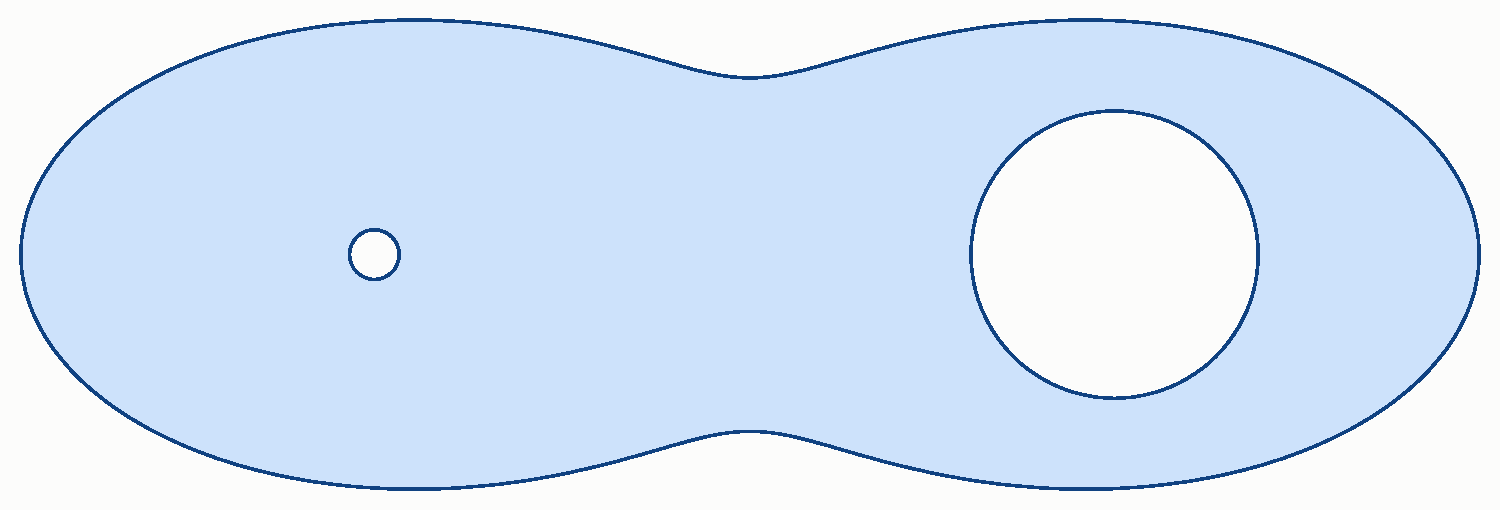
\includegraphics[width=1.00\textwidth]{figures/01_face.pdf}
\caption{The example face used throughout: a curved outline with an inward waist and two holes, about 260 $\times $ 176 mm, 166 cm$^2$ in area.}
\end{figure}
 

\section{Conventions and tolerances}
 

Points are pairs ($x$, $y$). A polygon is a list of points without a repeated closing point. Lengths are in centimetres throughout, because that is the unit the host program works in; this document quotes millimetres where a size is easier to picture that way. 

A \textbf{region} is a list of loops. Outlines run counter-clockwise and holes run clockwise, so the material always lies to the left of every loop. This single convention is what lets the same routine shrink an outline and grow a hole. 

The signed area of a polygon with points $p_{1}$\ldots{}$p_{n}$ is 
\begin{equation}
A = \frac12 \sum_i \bigl(x_i\,y_{i+1} - x_{i+1}\,y_i\bigr)
\end{equation}
 

positive for counter-clockwise order. Its centroid uses the same cross products: 
\begin{equation}
c_x = \frac{1}{6A} \sum_i (x_i + x_{i+1})\bigl(x_i\,y_{i+1} - x_{i+1}\,y_i\bigr),\qquad \text{and likewise for } c_y
\end{equation}
 

\begin{center}
\begin{tabular}{>{\raggedright\arraybackslash}p{0.24\textwidth}r>{\raggedright\arraybackslash}p{0.5\textwidth}}
\toprule
Tolerance & Value & Used for \\
\midrule
Merge distance & 0.001 mm & Points closer than this become one point \\
Straightness & 0.0001 mm & A point this close to the line through its neighbours is dropped \\
Curve sampling & 0.02 mm & How far the sampled points of a curved edge may lie from the true curve \\
Round-join sampling & 0.005 mm & How far the straight pieces of a rounded offset corner may lie from the true arc \\
Snap distance & 0.000001 mm & Points this close are treated as identical when pieces of outline are joined \\
Small turn & 12$^\circ $ & Corners turning less than this get no arc when a pocket is rounded \\
\bottomrule
\end{tabular}
\end{center}
 

Every polygon that comes out of a calculation passes through a cleaning step: repeated points are removed, then points that lie on the line through their neighbours, and a polygon left with fewer than three points or with no area is discarded. 

\section{The outline of the face}
 

Each edge of the face, whether straight, an arc or a free-form curve, is sampled into a chain of points that stays within 0.02 mm of the true edge. A straight edge gives two points. A circle of 30 mm radius gives about 85. 

The chains of one loop arrive in no particular order and direction. They are joined greedily: starting from the first chain, the routine repeatedly looks for the unused chain with an end nearest to the current end, reverses it if needed, and appends it. A loop that consists of a single closed edge, such as a round hole, has its repeated closing point removed. 

The points are then expressed in a flat coordinate system that lies in the face: an origin, two unit vectors $\mathbf{u}$ and $\mathbf{v}$ at right angles, and the normal $\mathbf{n}$ = $\mathbf{u}$ $\times $ $\mathbf{v}$. A point $\mathbf{p}$ in space becomes 
\begin{equation}
x = (\mathbf{p} - \mathbf{o})\cdot\mathbf{u}, \qquad y = (\mathbf{p} - \mathbf{o})\cdot\mathbf{v}
\end{equation}
 

From here on the problem is two-dimensional. The pattern is calculated once in this frame and reused for as long as the face and the settings stay the same. 

\section{Shrinking a region}
 

Three steps of the method need the face shrunk by some distance $d$: the usable area (shrunk by the margin), the rounding step (shrunk by margin plus corner radius) and the minimum-width filter. Shrinking means that every point of the result is at least $d$ away from every edge of the face. The outline moves inward and the holes grow. 

\subsection{Moving one loop}
 

Each loop is moved by $d$ to its left, which is the material side. Every edge is shifted along its left normal. What happens at a corner depends on the direction of the turn there. 
\begin{itemize}
 
\item \textbf{Left turn} (the material bends inward, an outward corner of the face): the two shifted edges overlap and are cut at the point where they meet. With unit left normals $\mathbf{n}_{1}$, $\mathbf{n}_{2}$ of the two edges and the corner at $\mathbf{v}$, that point is 
\begin{equation}
\mathbf{m} = \mathbf{v} + d\,\frac{\mathbf{n}_1 + \mathbf{n}_2}{1 + \mathbf{n}_1\cdot\mathbf{n}_2}
\end{equation}
 The corner stays sharp, which is exact: the point of the shrunk region nearest to an outward corner is that mitre point. 
\item \textbf{Right turn} (an inward corner of the face, or any corner of a hole): the shifted edges leave a gap, which is closed by an arc of radius $d$ around the corner. This too is exact, since the points at distance $d$ from a corner form a circle. 
\end{itemize}
 

The arc is drawn with straight pieces. The number of pieces follows from the allowed deviation $\varepsilon $ = 0.005 mm: a chord across an angle $\theta $ of a circle of radius $d$ lies $d$(1 $-$ cos($\theta $/2)) inside it, so the largest step is 
\begin{equation}
\theta_{\max} = 2\arccos\!\left(1 - \frac{\varepsilon}{d}\right), \qquad \text{capped at } 15^\circ
\end{equation}
 

One detail matters for correctness. Chords cut inside the arc, which would bring the shrunk region slightly closer than $d$ to the corner. The corners of the straight pieces are therefore placed just outside the arc, at radius $d$ / cos($\theta $/2), so that the pieces touch the arc from outside. The result errs on the safe side: a pocket is never closer to an edge than the margin. An early version placed the points on the arc, and four tests failed by a few thousandths of a millimetre until this was changed. 

\subsection{Cleaning up}
 

Where the face is narrower than 2$d$, the moved loop crosses itself. The crossings are found with a grid: every edge is entered into the grid squares its bounding box touches, and only pairs sharing a square are tested. Each crossing splits the loop in two, and the splitting repeats until no loop crosses itself. 

Two checks decide which pieces are real: 
\begin{itemize}
 
\item \textbf{Direction.} A real piece runs the same way round as the loop it came from. A fold, such as the sliver where a narrow neck has closed, runs the other way and is dropped. 
\item \textbf{Distance.} Just inside the three longest edges of the piece, the distance to the original loop must be at least $d$. 
\end{itemize}
 

The result can have a different number of loops than the input: a neck narrower than 2$d$ pinches the outline in two, and a part thinner than 2$d$ disappears. Grown holes may overlap each other or reach beyond the shrunk outline. This is left as it is; the inside test of the next section handles it. 

\begin{figure}[H]
\centering
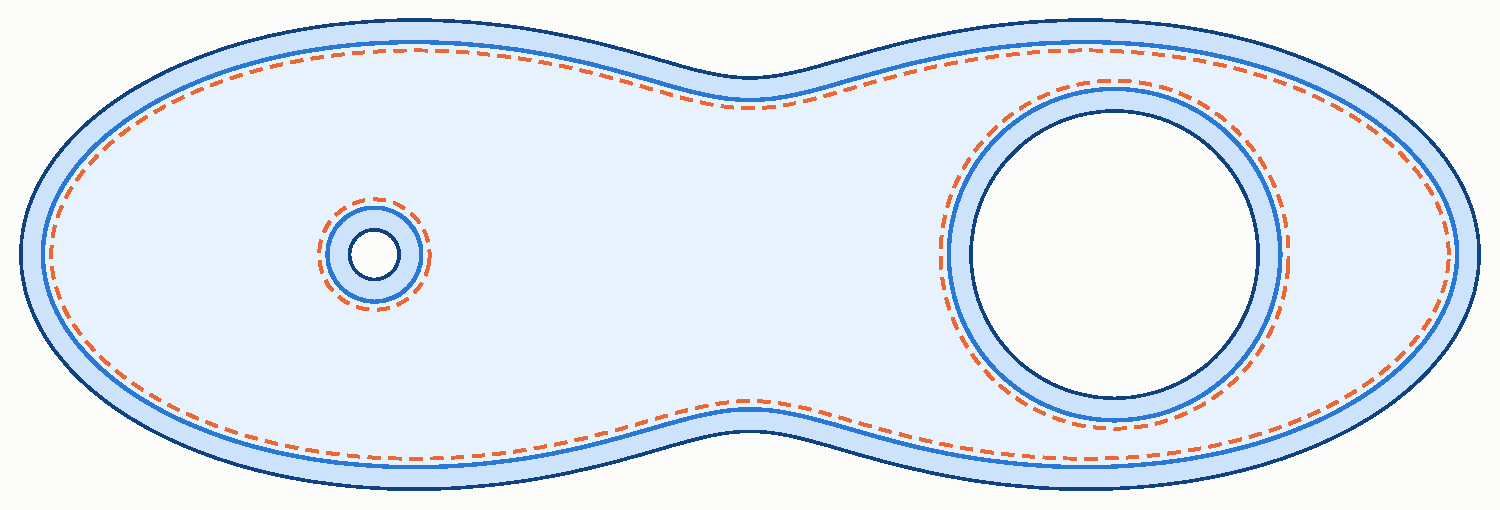
\includegraphics[width=1.00\textwidth]{figures/02_shrunk.pdf}
\caption{The face shrunk by the 4 mm margin (solid line, the usable area, 134 of 166 cm$^2$) and by margin plus corner radius (dashed). The outline has moved inward and both holes have grown.}
\end{figure}
 

\section{Inside tests}
 

Many steps ask whether a point lies inside a region. The answer comes from the winding number: the number of outlines around the point minus the number of holes around it. A point is inside when that number is positive. This definition gives the right answer where grown holes overlap (the count there is $-$1, still not inside) and where a hole reaches past the outline. 

The winding number is found by sending a ray from the point to the right and counting the edges it crosses: plus one for an edge going upward with the point on its left, minus one for an edge going downward with the point on its right. 

To make this fast, the edges of a region are indexed once. The region's bounding box is divided into a grid of about $\surd n$ by $\surd n$ squares for $n$ edges. Each edge is entered into the rows it spans, so that a winding query looks only at the edges of one row, and into the squares it touches, so that "which edges come near this box" is answered without looking at the rest. 

\section{Seed points}
 

Seeds are drawn at random, uniformly over the bounding box of the face, and kept only if they fall inside the usable area. The random generator is seeded with the user's seed value, so the same seed always produces the same pattern. Sampling stops after the requested number of points, or after 200 attempts per point on faces that are hard to hit. 

When the cells are meant to differ in size (section 16), a second test thins the points: a candidate at $\mathbf{x}$ is kept with probability $\rho $($\mathbf{x}$) / $\rho _{\mathrm{max}}$, where $\rho $ is the wanted number of cells per area. 

\section{Voronoi cells}
 

The Voronoi cell of a seed $\mathbf{p}$ is the set of points closer to $\mathbf{p}$ than to any other seed. For one other seed $\mathbf{q}$, "closer to $\mathbf{p}$" is a half-plane bounded by the line halfway between them: 
\begin{equation}
(\mathbf{q} - \mathbf{p})\cdot\mathbf{x} \;\le\; \frac{|\mathbf{q}|^2 - |\mathbf{p}|^2}{2}
\end{equation}
 

The cell is the intersection of these half-planes over all other seeds. The add-in builds it exactly that way. The cell starts as the bounding box and is cut by one half-plane after another. Cutting a convex polygon by a half-plane is a walk around its corners: corners on the kept side stay, and where an edge crosses the line, the crossing point is inserted. 

Cutting by every other seed would cost a number of steps proportional to the square of the number of seeds per cell. An early stop avoids most of it. The other seeds are visited from nearest to farthest. The halfway line to a seed at distance $\delta $ lies $\delta $/2 from $\mathbf{p}$. If $R$ is the distance from $\mathbf{p}$ to the farthest corner of the cell so far, then once 
\begin{equation}
\delta > 2R
\end{equation}
 

the line passes outside the cell, and so does every later one. On evenly spread seeds the loop stops after roughly 15 to 20 neighbours regardless of the total. 

This approach was chosen over the usual triangulation-based algorithms because it has no special cases. Every cell is the result of cutting one convex polygon, so it is always a valid convex polygon, and seeds on a common circle or in a line need no extra handling. An exact duplicate of a seed gets an empty cell. 

\section{Evening out the cells}
 

Random seeds give cells of very different sizes. Lloyd's algorithm evens them out: each seed is moved to the centroid of its own cell, the cells are recomputed, and this is repeated. The cell is first trimmed to the usable area (section 10), so the centroid is that of the part that will actually hold a pocket. Seeds therefore spread out evenly right up to the border and around holes, instead of being pulled toward the empty space outside the face. 

A move is accepted only if the new position is inside the usable area. On the example face the spread of cell areas (standard deviation divided by mean) falls from 74\% for the raw seeds to 49\% after the default two passes and 30\% after eight. The first passes do most of the work, which is why the default is low; the remaining unevenness is what makes the pattern look organic. 

\begin{figure}[H]
\centering
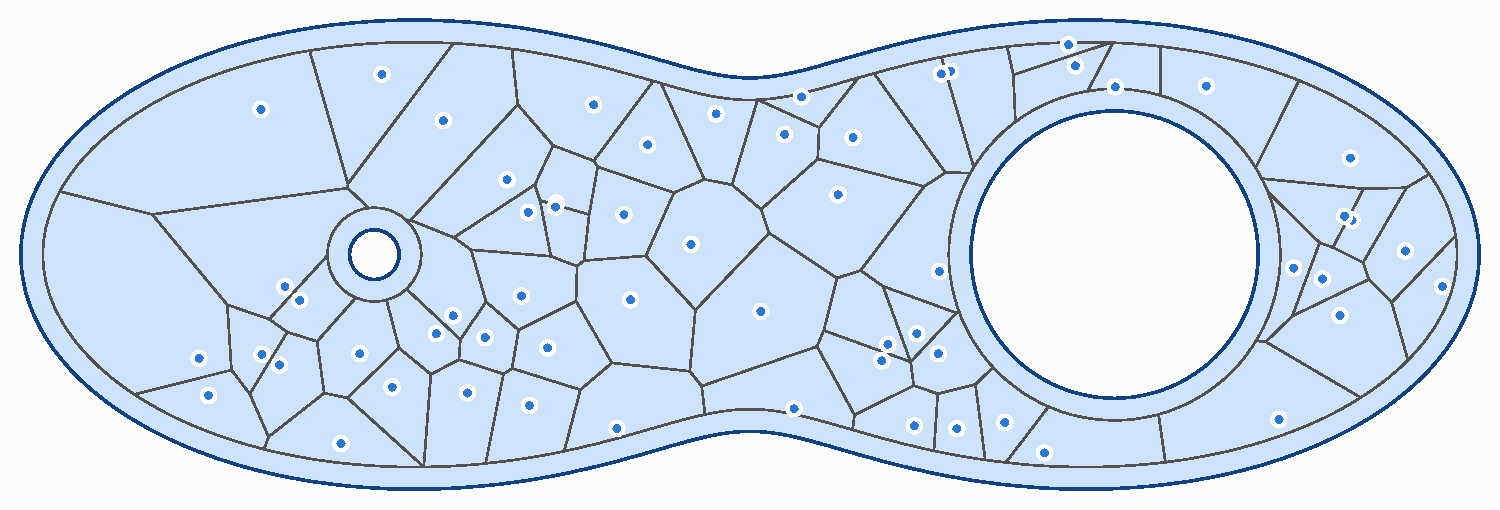
\includegraphics[width=0.480\textwidth]{figures/03_seeds_random.pdf}\hfill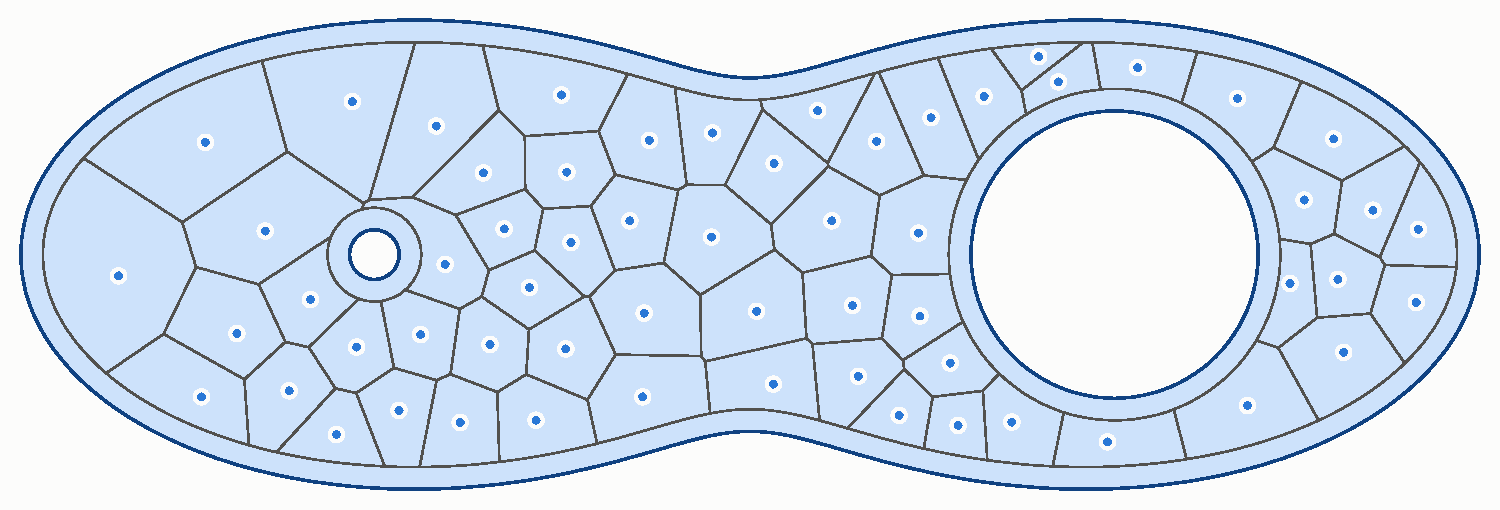
\includegraphics[width=0.480\textwidth]{figures/04_seeds_relaxed.pdf}
\caption{Sixty seeds and their cells, trimmed to the usable area. Left: as drawn at random. Right: after two smoothing passes.}
\end{figure}
 

\begin{figure}[H]
\centering
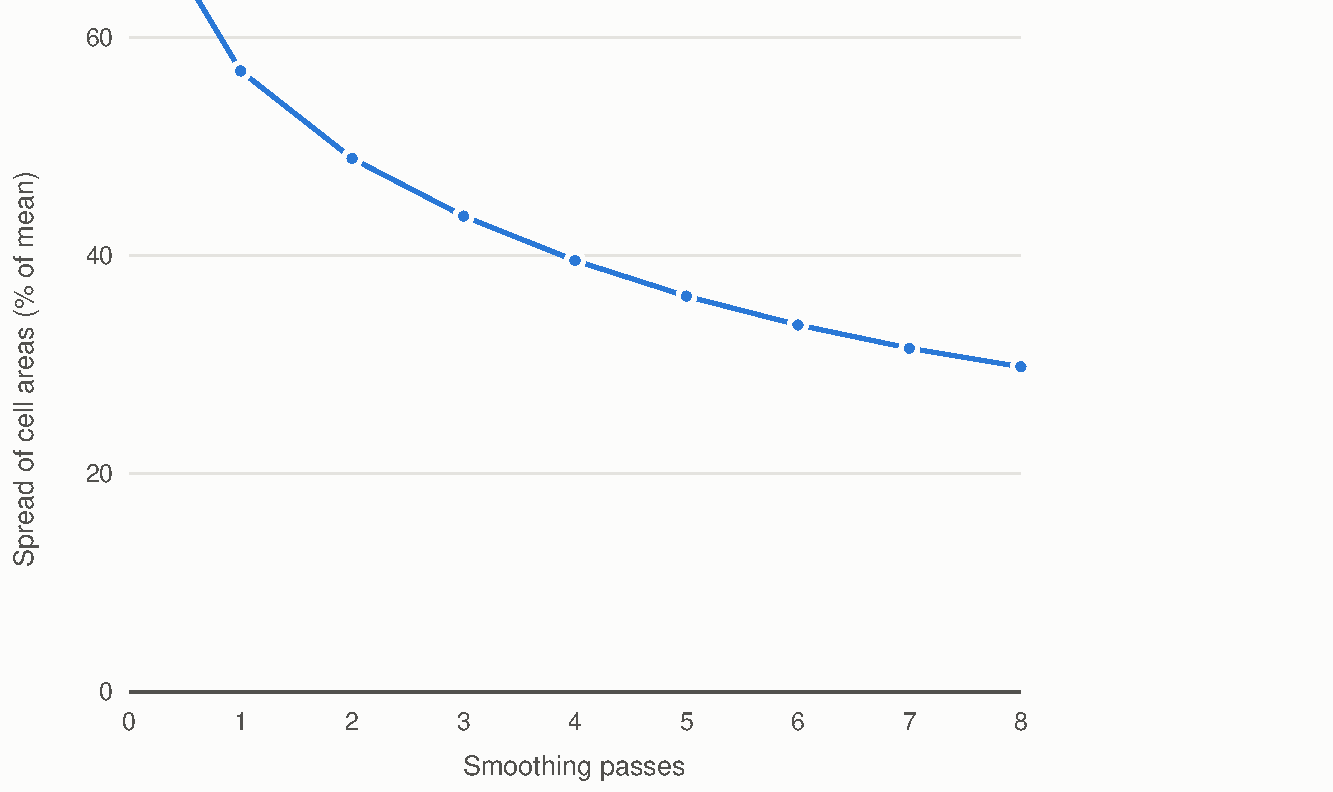
\includegraphics[width=0.80\textwidth]{figures/c_lloyd.pdf}
\caption{Spread of cell areas against the number of smoothing passes, for the sixty seeds of Figure 3.}
\end{figure}
 

\section{From a cell to a pocket}
 

The pocket of a cell is defined by three operations: shrink the cell by half the wall thickness $w$, cut it back to the face shrunk by the margin $m$, and round every corner to the radius $r$. 

Rounding is done in the exact way known from image processing as an opening: shrink the shape by $r$, then grow it back by $r$. Shrinking removes everything a circle of radius $r$ cannot reach; growing back restores the reachable part with every outward corner now an arc of exactly that radius. This is also precisely the area a milling tool of radius $r$ can clear. 

Shrinking distributes over intersection, so the shrink can be applied to the cell and to the face separately: 
\begin{equation}
\text{core} = \operatorname{shrink}\bigl(\text{cell},\, \tfrac{w}{2} + r\bigr) \;\cap\; \operatorname{shrink}\bigl(\text{face},\, m + r\bigr)
\end{equation}
 
\begin{equation}
\text{pocket} = \operatorname{grow}(\text{core},\, r)
\end{equation}
 

Three guarantees follow directly from this form. 
\begin{itemize}
 
\item \textbf{Walls.} Two neighbouring cells share an edge. Their cores are at least $w$ + 2$r$ apart, and each grows by $r$, so the rib between two pockets is at least $w$ thick, and exactly $w$ along the straight part of the shared edge. 
\item \textbf{Border.} The core stays $m$ + $r$ from every edge of the face and grows by $r$, so the pocket stays at least $m$ away, and exactly $m$ wherever it follows the border. 
\item \textbf{Corners.} Every outward corner of every pocket has radius exactly $r$, including the corners where a pocket meets the border line. 
\end{itemize}
 

Shrinking a convex polygon is simple: each edge is moved inward by the distance and the polygon is cut by the half-plane of the moved edge, using the same cutting routine as the Voronoi step. If nothing is left, the cell is too small and gives no pocket. 

\begin{figure}[H]
\centering
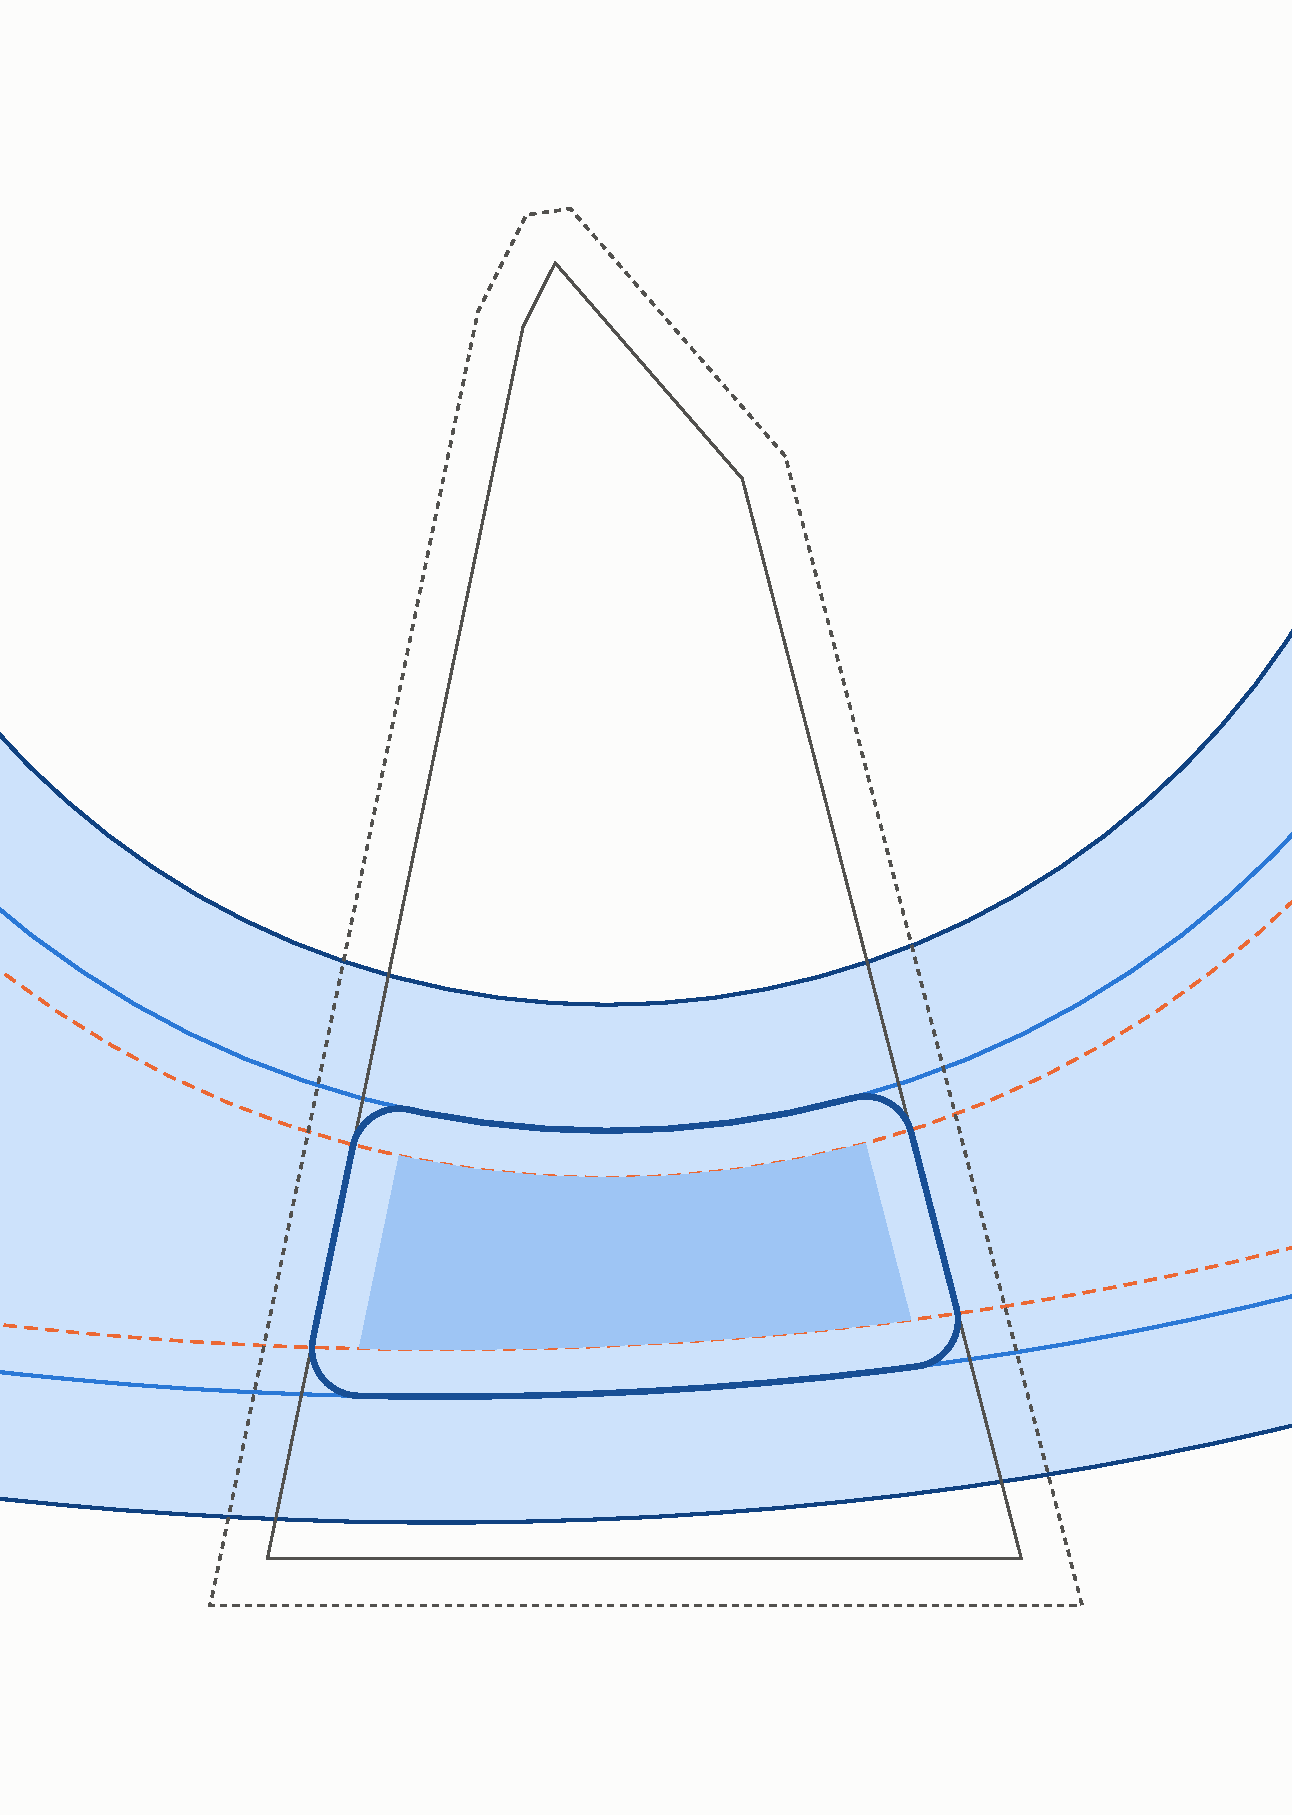
\includegraphics[width=1.00\textwidth]{figures/05_one_cell.pdf}
\caption{One cell at the inward waist of the face. Dotted: the Voronoi cell. Thin line: the cell shrunk by half the wall. Solid blue line: the border of the usable area. Dashed orange: the face shrunk by margin plus radius. Light fill: the core. Heavy outline: the finished pocket, the core grown back by the corner radius. Along the border the pocket follows the curve of the face.}
\end{figure}
 

\section{Trimming a cell to the face}
 

Equation (8) needs the intersection of a convex polygon (the shrunk cell) with a region that can be any shape, can have holes, and whose loops can overlap. The result can be several pieces, and it can have a hole in it. 

Most cells never reach this code. If no edge of the region comes near the cell's bounding box, the cell is either wholly inside or wholly outside, and one inside test of its centroid settles it. 

For the others the routine works with pieces of outline: 
\begin{enumerate}
 
\item Every nearby edge of the region is cut down to the part inside the cell. For a segment from $\mathbf{a}$ to $\mathbf{b}$ and each edge of the convex cell with outward normal $\mathbf{n}$ through point $\mathbf{q}$, the parameter $t$ = $\mathbf{n}\cdot $($\mathbf{q}$ $-$ $\mathbf{a}$) / $\mathbf{n}\cdot $($\mathbf{b}$ $-$ $\mathbf{a}$) is where the segment crosses that edge's line. It bounds the kept part from above if the segment is leaving and from below if it is entering. 
\item Where pieces of two different loops cross inside the cell, both are split at the crossing. 
\item The cell's own edges are split wherever a region edge starts or ends on them. 
\item Each piece is kept or dropped. A piece of the cell's outline is kept if its midpoint is inside the region. A piece of a region loop is kept if the other loops do not already decide the matter: the winding number of all other loops at its midpoint must be 0 for an outline and 1 for a hole. 
\item The kept pieces are joined head to tail into closed loops. 
\end{enumerate}
 

Every kept piece has "inside both" on its left and "not inside both" on its right, so the loops come out with the right orientation: counter-clockwise for outlines and clockwise for a hole of the region that lies wholly inside the cell. 

When only one loop of the region passes through the cell, which is the usual case, the answer of step 4 is the same for all of that loop's pieces and is computed once. With several loops it can only change where two loops cross, so it is carried along each unbroken run. These two shortcuts cut the number of inside tests by a large factor on cells that contain long stretches of a curved outline. 

\subsection{Cells around a hole}
 

A pocket that surrounds a hole would be a ring, with an island of material in the middle. To avoid this, a cell is checked before trimming: if a grown hole lies wholly inside the shrunk cell, the cell is cut in two by a straight line through the hole's centre, across the cell's longer side. Each half is then treated as a cell of its own, which gives two ordinary pockets with a normal wall between them. 

\subsection{Minimum pocket width}
 

A piece is kept only if a circle of the minimum width $w_{\mathrm{min}}$ fits inside it. That is the same question as whether the piece survives shrinking by $w_{\mathrm{min}}$/2, so it is answered by repeating equation (8) with $w_{\mathrm{min}}$/2 in place of $r$ and checking that something remains inside the piece. When the minimum width is not larger than twice the corner radius, the test is already implied by the core being non-empty and is skipped. 

\section{Rounding the corners}
 

Growing the core by $r$ moves every edge outward by $r$ along its outward normal. At each corner, with the turning angle $\theta $ measured positive for an outward corner, one of three things happens. 

\begin{center}
\begin{tabular}{>{\raggedright\arraybackslash}p{0.27\textwidth}>{\raggedright\arraybackslash}p{0.65\textwidth}}
\toprule
Corner & Result \\
\midrule
Outward, $\theta $ $\ge $ 12$^\circ $ & An arc of radius $r$ centred on the corner, from the end of one moved edge to the start of the next. It is stored by its start, middle and end points. \\
Outward, $\theta $ < 12$^\circ $ & A single point at distance $r$ from the corner along the bisector. It lies on the arc that would otherwise be drawn, so the pocket is never larger than the exact shape. \\
Inward & The two moved edges are extended until they meet, as in equation (4). The corner stays sharp. \\
\bottomrule
\end{tabular}
\end{center}
 

The second case exists for curved borders. Where a pocket follows a curved edge, its core has a small corner at every sample point of the curve, each turning a few degrees. An arc at each would double the number of curves for no visible gain. Replacing a 12$^\circ $ arc by a point shortens the outline by at most $r$(1 $-$ cos 6$^\circ $), which is 0.5\% of the radius. 

Inward corners of a core come only from inward-curving parts of the shrunk face. Those have a radius of curvature of at least $m$ + $r$, so growing by $r$ leaves a radius of at least $m$ and the moved edges cannot fold over. 

The area of a finished pocket is computed exactly: the area of the polygon through the start points of all its segments by equation (1), plus, for every arc of sweep $\varphi $, the sliver between the arc and its chord: 
\begin{equation}
A_{\mathrm{sliver}} = \frac12\, r^2\,(\varphi - \sin\varphi)
\end{equation}
 

\section{Results}
 

\begin{figure}[H]
\centering
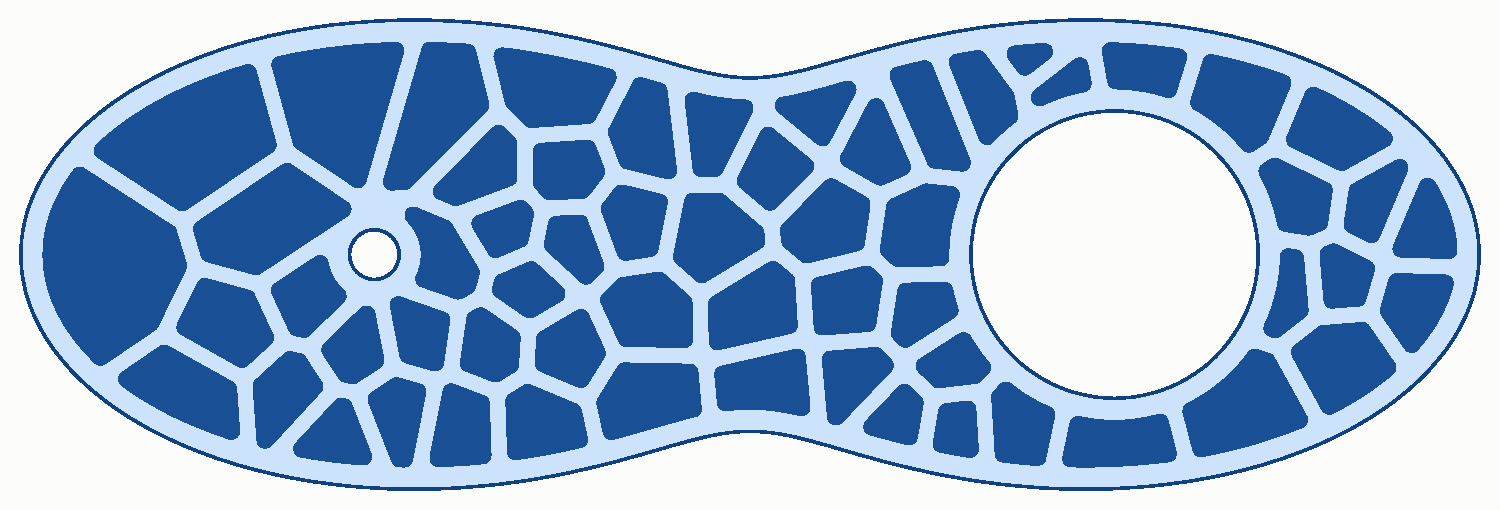
\includegraphics[width=1.00\textwidth]{figures/06_pattern_curved.pdf}
\caption{Sixty cells on the example face: wall 3 mm, margin 4 mm, corner radius 1.5 mm. The pockets cover 56.8\% of the face. The band along the outline and around both holes is 4 mm wide wherever a pocket reaches it.}
\end{figure}
 

\begin{figure}[H]
\centering
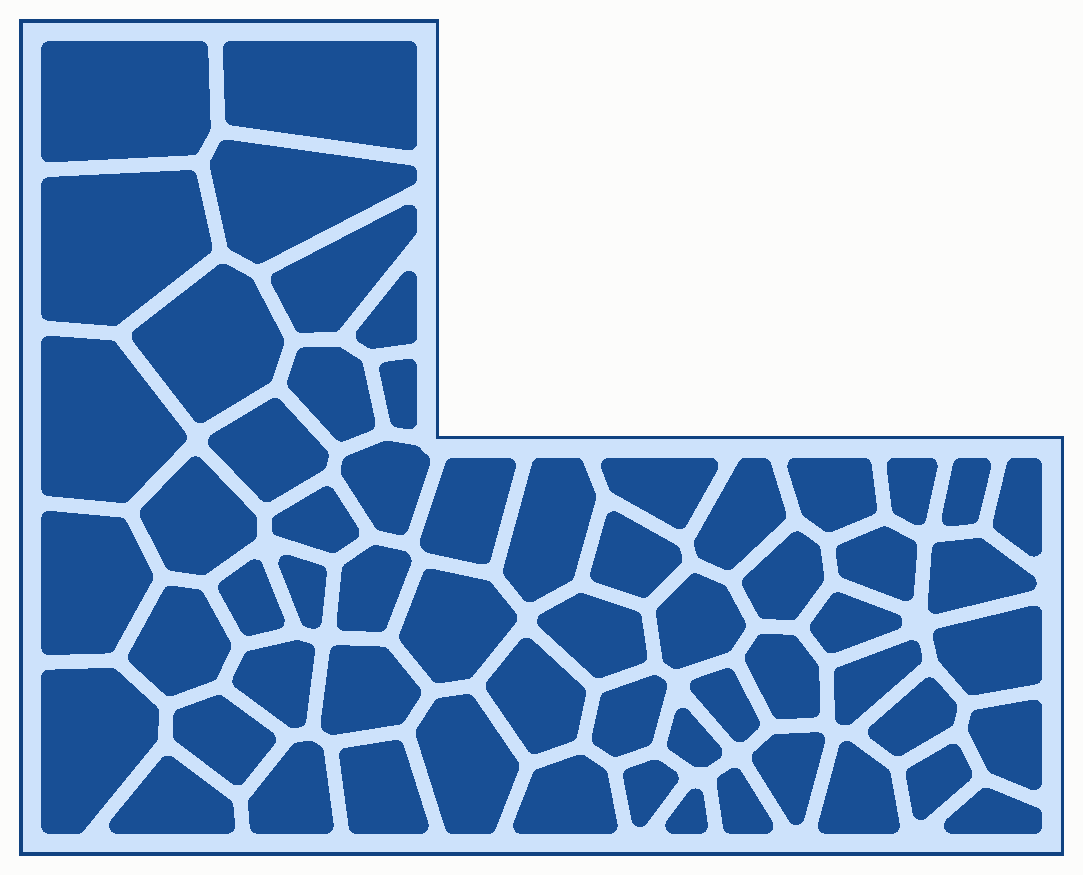
\includegraphics[width=0.70\textwidth]{figures/07_pattern_l.pdf}
\caption{An L-shaped face. At the inward corner the border band follows the corner in an arc, because the shrunk face has a round corner there.}
\end{figure}
 

\begin{figure}[H]
\centering
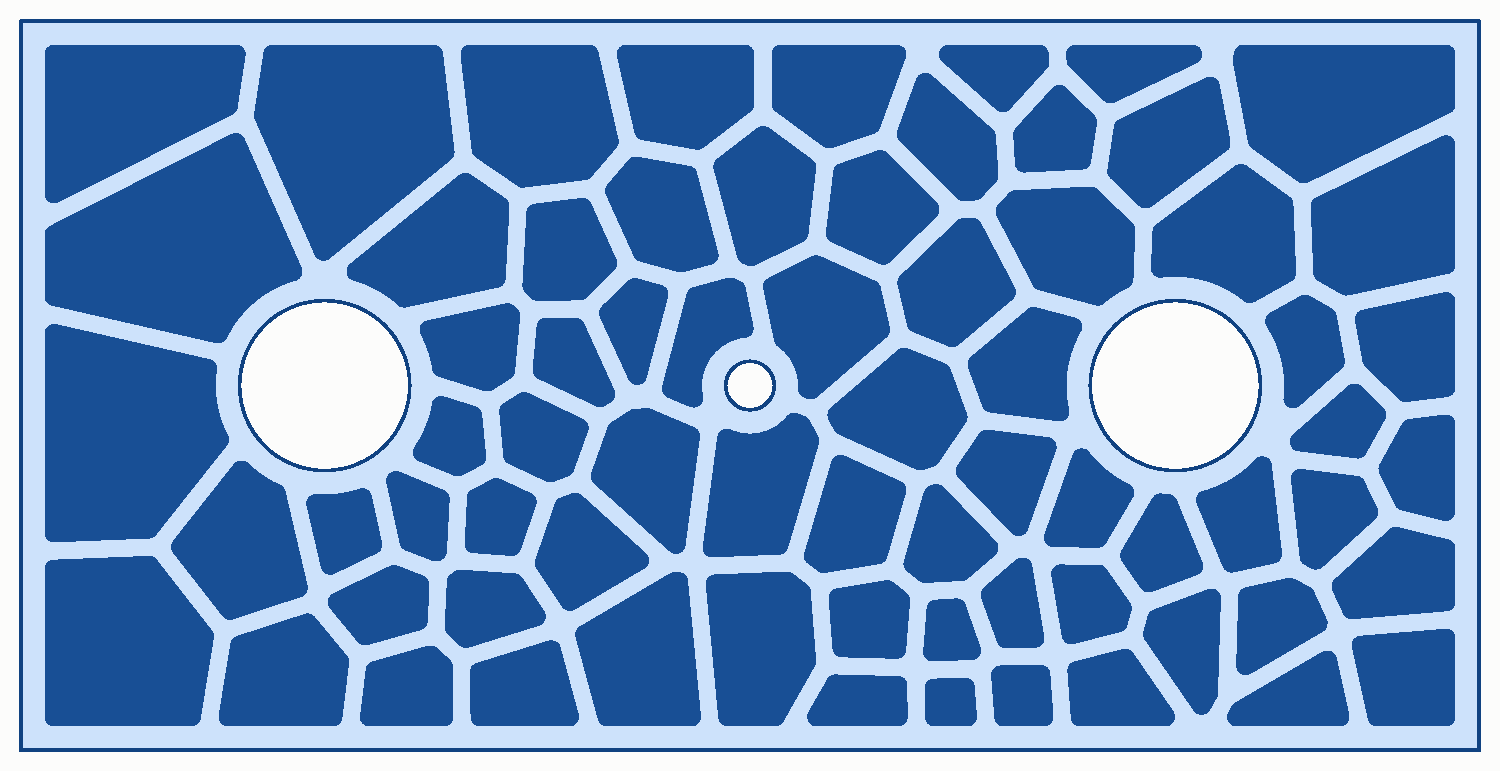
\includegraphics[width=1.00\textwidth]{figures/08_pattern_holes.pdf}
\caption{A plate with three holes. Each hole keeps a ring of the margin width. The cell that contained the small hole in the middle was split through it.}
\end{figure}
 

\section{Simple mode}
 

In simple mode the user gives only the border margin and the share $P$ of the face that should become pocket. The add-in chooses the number of cells, the wall thickness and the corner radius. 

There are more unknowns than conditions, so two are fixed by a rule. The corner radius is 8\% of the cell size, and pockets narrower than 25\% of the cell size are left out, where the cell size is $s$ = $\surd $($A_{\mathrm{usable}}$ / $N$) for $N$ cells. The remaining freedom, the trade between many thin-walled cells and few thick-walled ones, is settled by a design rule: the walls should be about as wide as the border margin, so that ribs and border look alike. 

\subsection{Wall thickness for a given number of cells}
 

The pocket area falls as the walls get thicker, so the wall that gives the wanted area $A_{\mathrm{w}}$ = $P$ $\cdot $ $A_{\mathrm{face}}$ can be found by a one-dimensional search. Each guess comes from a model: a cell that loses a strip of wall on every side keeps the share (1 $-$ $w$/$S$)$^2$ of its area, for some effective size $S$. With $A_{0}$ the pocket area at the thinnest wall $w_{0}$ (2\% of the cell size), the model is 
\begin{equation}
A(w) \approx A_0 \left(1 - \frac{w - w_0}{S}\right)^{2}
\end{equation}
 

which is solved for the next guess, 
\begin{equation}
w = w_0 + S\left(1 - \sqrt{A_{\mathrm{w}} / A_0}\right)
\end{equation}
 

After each trial the real pocket area is measured and $S$ is refitted through that point. The search keeps a bracket (one wall that gives too much pocket and one that gives too little); a guess that falls outside it is replaced by its middle. It stops when the area is within 0.05\% of the face, typically after three or four trials. Only the last three steps of the method (shrink, trim, round) are repeated per trial; the seeds and cells are reused. 

\subsection{Number of cells}
 

The first guess uses the same model with $w$ set to the margin: the pockets must fill the share $A_{\mathrm{w}}$/$A_{\mathrm{usable}}$ of the usable area, which gives a cell size and from it a count. After the wall for that count has been found, the count is corrected. Wall thickness scales with cell size, and cell size with 1/$\surd N$, so 
\begin{equation}
N_{\mathrm{new}} = N \left(\frac{w}{m}\right)^{2}
\end{equation}
 

The loop ends when the wall is within 10\% of the margin, when the count hits its limits of 5 and 120, or after six rounds. If the share cannot be reached even with the thinnest wall, the count is reduced by 40\% per round, since fewer, larger cells waste less area on walls; if it is still out of reach, the result with the most pocket is returned and reported as such. 

\begin{figure}[H]
\centering
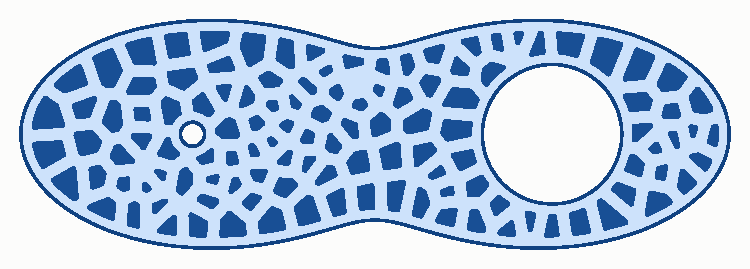
\includegraphics[width=0.320\textwidth]{figures/09_simple_30.pdf}\hfill
\includegraphics[width=0.320\textwidth]{figures/09_simple_50.pdf}\hfill
\includegraphics[width=0.320\textwidth]{figures/09_simple_70.pdf}
\caption{Simple mode with a 4 mm margin at 30\%, 50\% and 70\%. Chosen: 120 cells with 4.9 mm walls, 58 cells with 4.2 mm walls, 11 cells with 4.3 mm walls. At 30\% the cell limit is reached, so the walls are thicker than the margin.}
\end{figure}
 

\begin{figure}[H]
\centering
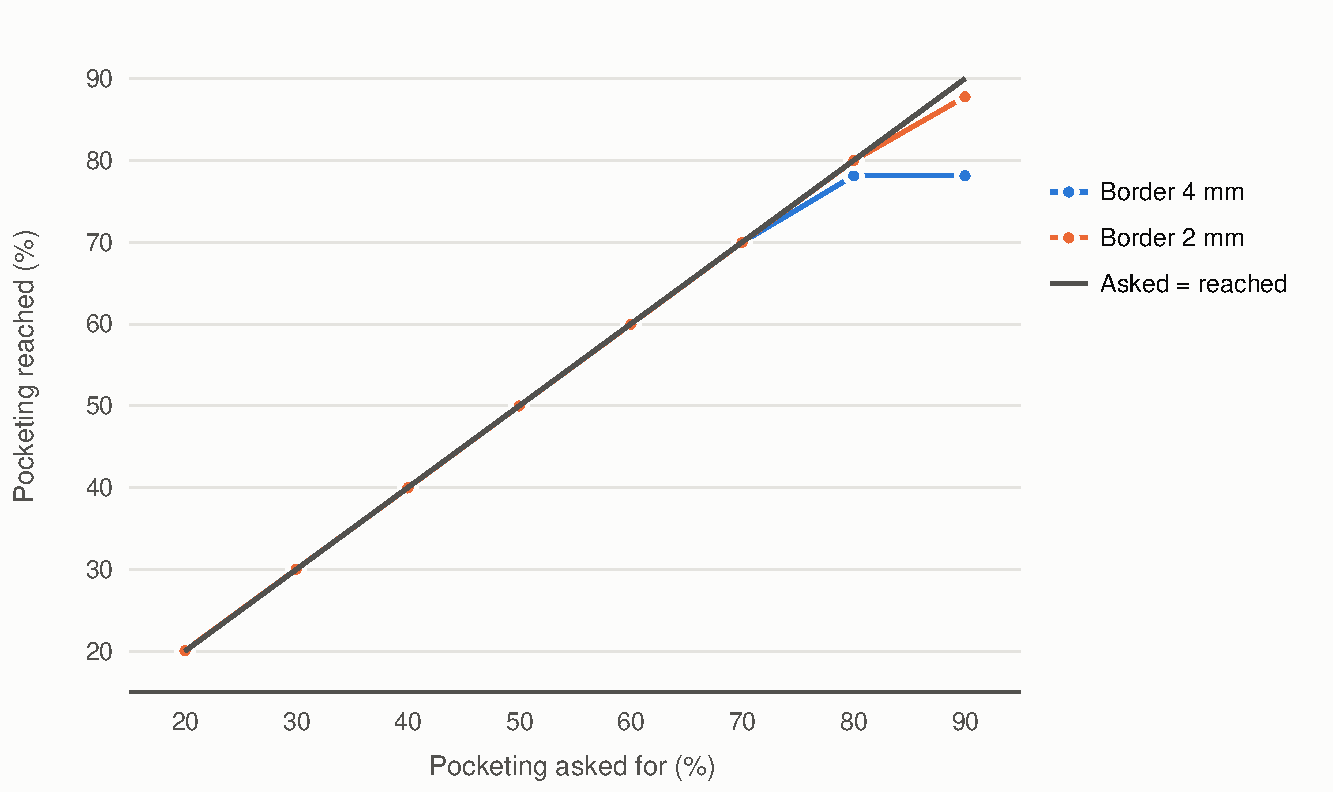
\includegraphics[width=0.80\textwidth]{figures/c_simple.pdf}
\caption{Pocketing reached against pocketing asked for, on the example face. With a 4 mm border the share levels off at 78.1\%: the border band and the rings around the holes alone take a fifth of this face. With a 2 mm border 80\% is reached and the limit is 87.8\%.}
\end{figure}
 

\section{The stress calculation}
 

The stress-driven mode treats the face as a thin flat plate that is held along some edges and loaded by forces within its own plane. This is the plane-stress model of linear elasticity. It answers one question: how hard is the solid plate working at each point? 

\subsection{Material law}
 

With strains $\varepsilon _{x}$, $\varepsilon _{y}$, $\gamma _{xy}$ and stresses $\sigma _{x}$, $\sigma _{y}$, $\tau _{xy}$, Young's modulus $E$ and Poisson's ratio $\nu $: 
\begin{equation}
\sigma_x = d_{11}\,\varepsilon_x + d_{12}\,\varepsilon_y, \qquad \sigma_y = d_{12}\,\varepsilon_x + d_{11}\,\varepsilon_y, \qquad \tau_{xy} = d_{33}\,\gamma_{xy}
\end{equation}
 
\begin{equation}
d_{11} = \frac{E}{1 - \nu^2}, \qquad d_{12} = \nu\, d_{11}, \qquad d_{33} = d_{11}\,\frac{1 - \nu}{2}
\end{equation}
 

For given forces the stress does not depend on $E$: a stiffer plate moves less under the same force but carries the same stress. The calculation therefore uses a fixed stiffness and takes only $\nu $ and the yield strength from the material. 

\subsection{Mesh}
 

The plate is divided into triangles of size $h$, by default the diagonal of the face divided by 65, which gives about 2,500 points. 

A pattern of equal-sided triangles is laid over the face: rows $h\cdot \surd $3/2 apart, every second row shifted by $h$/2. Points of the pattern near the border are then moved onto it: 
\begin{itemize}
 
\item A point closer than 0.51 $h$ to the border moves to its nearest border point. The factor just over one half guarantees that of two neighbouring points on opposite sides of the border at least one is moved, so the rim of the mesh consists of moved points only and follows the outline exactly. 
\item Moved points that land within 0.3 $h$ of each other become one point. Without this, the thin triangle between them would have to be dropped, which leaves a slit in the mesh that behaves like a crack. 
\item For every corner of the face that turns by more than 25$^\circ $, the nearest border point within 0.75 $h$ is placed exactly on the corner. 
\end{itemize}
 

A triangle is kept if its three points are distinct, if it has not been flattened or flipped by the moving (its area is at least 2\% of a full triangle's), and if its centroid is inside the face. Of what remains, only the largest group of triangles joined edge to edge is used: a fragment hanging on by one corner could turn freely and would make the equations unsolvable. 

On the test shapes the mesh reproduces the area of the face to within 0.2\%, every rim edge lies on the true border, and the least regular triangle has a quality of 0.59 on a scale where an equal-sided triangle scores 1. 

\begin{figure}[H]
\centering
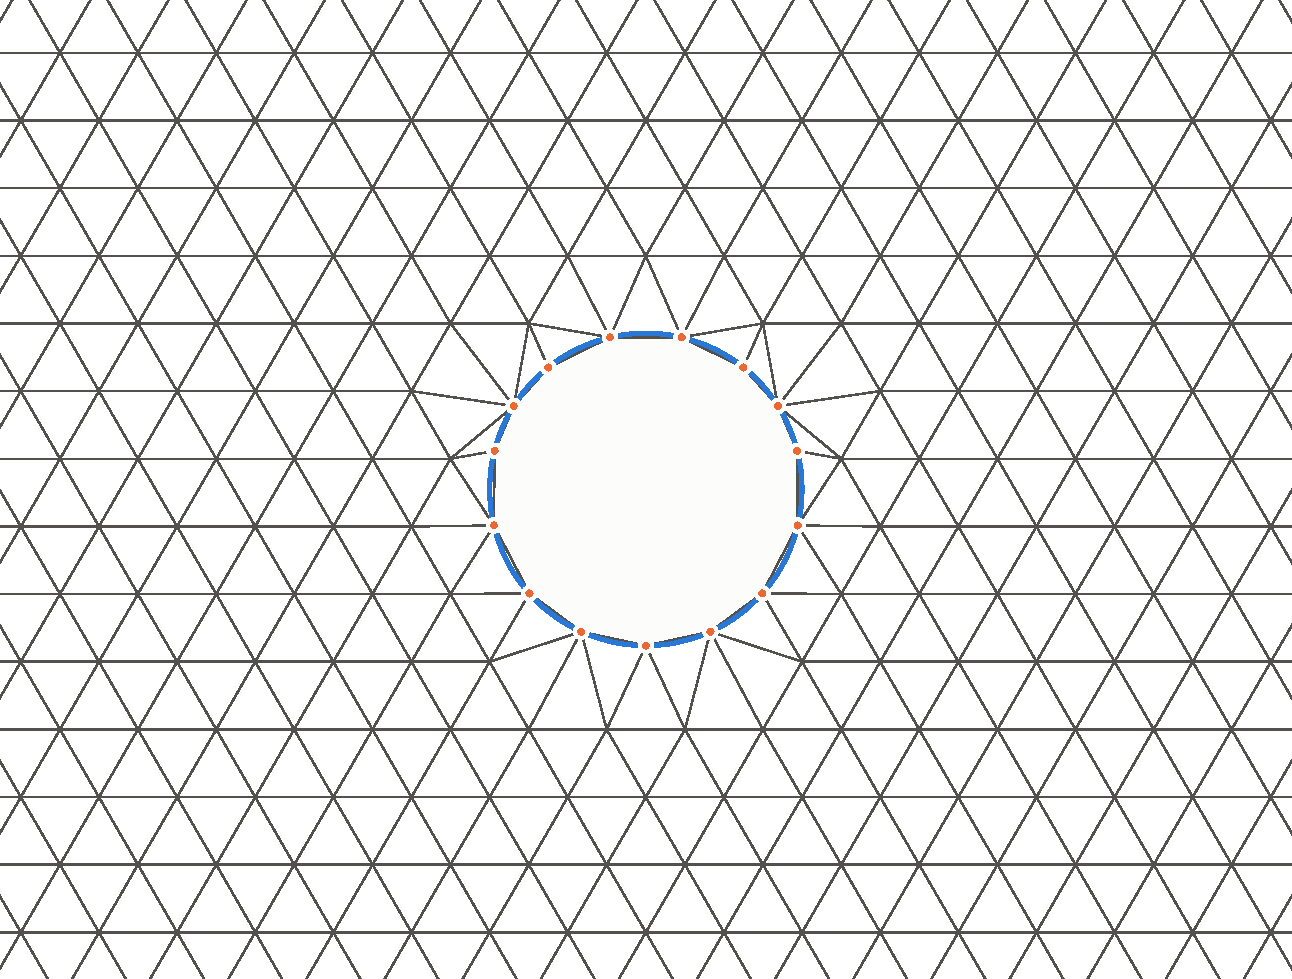
\includegraphics[width=1.00\textwidth]{figures/10_mesh.pdf}
\caption{The mesh around a round hole at two triangles per hole radius. Orange points were moved onto the border.}
\end{figure}
 

\subsection{Stiffness of one triangle}
 

Each triangle has corners 1, 2, 3 in counter-clockwise order. Inside it the displacement varies linearly, so the strain is the same everywhere in the triangle. With cyclic indices define 
\begin{equation}
b_i = y_j - y_k, \qquad c_i = x_k - x_j, \qquad 2A = x_1 b_1 + x_2 b_2 + x_3 b_3
\end{equation}
 

The strains follow from the corner displacements ($u_{i}$, $v_{i}$): 
\begin{equation}
\varepsilon_x = \frac{1}{2A}\sum_i b_i u_i, \qquad \varepsilon_y = \frac{1}{2A}\sum_i c_i v_i, \qquad \gamma_{xy} = \frac{1}{2A}\sum_i \bigl(c_i u_i + b_i v_i\bigr)
\end{equation}
 

The stiffness that links the forces at corner $p$ to the displacements of corner $q$, for a plate of thickness $t$, is the 2 $\times $ 2 block 
\begin{equation}
\mathbf{K}_{pq} = \frac{t}{4A} \begin{pmatrix} d_{11}\,b_p b_q + d_{33}\,c_p c_q & d_{12}\,b_p c_q + d_{33}\,c_p b_q \\[3pt] d_{12}\,c_p b_q + d_{33}\,b_p c_q & d_{11}\,c_p c_q + d_{33}\,b_p b_q \end{pmatrix}
\end{equation}
 

The blocks of all triangles are added into one table with two rows per mesh point. It is stored row by row, each row holding only its non-zero entries, about fourteen. 

\subsection{Supports and forces}
 

\textbf{Held edges.} Every mesh point on a held edge is fixed in both directions, and its two rows are removed from the equations. At least three fixed directions are needed, since a flat body can otherwise slide two ways and turn. 

\textbf{Force on an edge.} The force is spread evenly along the edge. Each mesh point on it receives the share of the edge it covers: half the distance to its neighbour on each side, divided by the total. On a closed rim, such as a hole, the gap between the last and the first point is split between them. With several loaded edges the force is divided by their lengths. 

\textbf{Force at a point.} A force placed on a single mesh point produces a stress spike whose height depends on the mesh and on nothing physical. A point force is therefore spread over the mesh points within 1.5 $h$ of its position, with weights that fall off linearly: 
\begin{equation}
w_k = 1 - \frac{\lVert \mathbf{x}_k - \mathbf{x}_0 \rVert}{1.5\,h}, \qquad \mathbf{f}_k = \mathbf{F}\,\frac{w_k}{\sum_j w_j}
\end{equation}
 

The weights add up to one, so the total force is exactly what was asked for. This models a force arriving through a bolt head or a small pad. 

\subsection{Solving}
 

The equations \textbf{K u} = $\mathbf{f}$ are solved by the conjugate gradient method. It needs only one operation on the table, multiplying it by a vector, which suits the row-by-row storage. Each step first divides the remaining error by the diagonal of $\mathbf{K}$, which evens out stiff and soft spots and reduces the number of steps. Starting from $\mathbf{u}$ = 0, $\mathbf{r}$ = $\mathbf{f}$, $\mathbf{z}$ = $\mathbf{r}$ / diag($\mathbf{K}$), $\mathbf{p}$ = $\mathbf{z}$, one step is 
\begin{equation}
\begin{aligned} \alpha &= \frac{\mathbf{r}\cdot\mathbf{z}}{\mathbf{p}\cdot\mathbf{K}\mathbf{p}}, & \mathbf{u} &\leftarrow \mathbf{u} + \alpha\,\mathbf{p}, & \mathbf{r} &\leftarrow \mathbf{r} - \alpha\,\mathbf{K}\mathbf{p}, \\ \mathbf{z} &\leftarrow \frac{\mathbf{r}}{\operatorname{diag}(\mathbf{K})}, & \mathbf{p} &\leftarrow \mathbf{z} + \frac{(\mathbf{r}\cdot\mathbf{z})_{\mathrm{new}}}{(\mathbf{r}\cdot\mathbf{z})_{\mathrm{old}}}\,\mathbf{p} \end{aligned}
\end{equation}
 

The loop ends when the length of $\mathbf{r}$ has fallen to one ten-millionth of the length of $\mathbf{f}$. As a check, the force the supports push back with is computed from the solution; it must equal the applied force with the opposite sign, and in every test it does to better than a thousandth of a newton. 

\subsection{Stress at the mesh points}
 

Equations (17) and (14) give one stress per triangle. Values at the mesh points are needed for a smooth field. 

For a point inside the plate, the stress is the average over the triangles around it, weighted by their areas. A point on the border has triangles on one side only, so an average reads too low exactly where stress peaks, such as beside a hole. For border points a sloping plane $s$ = $a$ + $b \xi $ + $c \eta $ is fitted by least squares through the stresses of the nearby triangles (those sharing a point with one of the point's own triangles), taken at their centroids, with $\xi $, $\eta $ measured from the point. The value at the point is $a$. The fit is used when at least five triangles are available. 

\subsection{One number for the load, and the safety factor}
 

The three stress components are combined into the von Mises stress, the usual measure for when a metal starts to yield: 
\begin{equation}
\sigma_{\mathrm{vM}} = \sqrt{\sigma_x^2 - \sigma_x\sigma_y + \sigma_y^2 + 3\,\tau_{xy}^2}
\end{equation}
 

With the yield strength $\sigma _{\mathrm{y}}$ of the material and a target safety factor $n_{\mathrm{t}}$ chosen by the user: 
\begin{equation}
n = \frac{\sigma_{\mathrm{y}}}{\sigma_{\mathrm{vM}}}, \qquad \sigma_{\mathrm{a}} = \frac{\sigma_{\mathrm{y}}}{n_{\mathrm{t}}}
\end{equation}
 

Inside a triangle the value is interpolated linearly from its three corners. Lengths are in centimetres and forces in newtons, so stresses come out in N/cm$^2$, and 1 MPa is 100 N/cm$^2$. 

For display, the face can be coloured by stress (position $\sigma _{\mathrm{vM}}$ / $\sigma _{\mathrm{a}}$ on the colour scale) or by safety factor. The safety scale is logarithmic, position 1 $-$ log$_{2}$($n$) / 3, so that each doubling of the safety factor moves the same distance: 1 or below at one end, 8 or above at the other. 

\section{Accuracy of the stress}
 

The calculation is checked against cases with a known answer. Two are exact by construction and three show the size of the error. 

\subsection{Even pull and pure shear}
 

A strip pulled evenly by a force $F$, free to narrow, must show $\sigma _{x}$ = $F$ / (height $\times $ thickness) everywhere and nothing else. The triangle used here can represent such a state exactly, and the result agrees to better than one part in a million, as do the stretch $FL$/($E$ $\times $ cross-section) and the narrowing by Poisson's ratio. A sheared rectangle gives the expected shear stress within 2\% away from its ends. These two cases confirm that equations (16) to (20) are implemented correctly. 

\subsection{A bent plate}
 

A plate 200 $\times $ 100 $\times $ 5 mm is held at its left edge and pushed down at its right edge with 1000 N. Beam theory gives a stress along the plate that varies linearly across the height, zero on the middle line: 
\begin{equation}
\sigma_x = \frac{F\,(L - x)\,y}{I}, \qquad I = \frac{t\,H^3}{12}
\end{equation}
 

Half-way along the plate the computed values lie on that line: the largest difference is 14 N/cm$^2$ where the edge value is 1,203 N/cm$^2$, about 1\%. On the middle line the stress is pure shear, 1.5 $F$ / ($H t$), giving a von Mises value of 520 N/cm$^2$; the calculation returns 520. 

\begin{figure}[H]
\centering
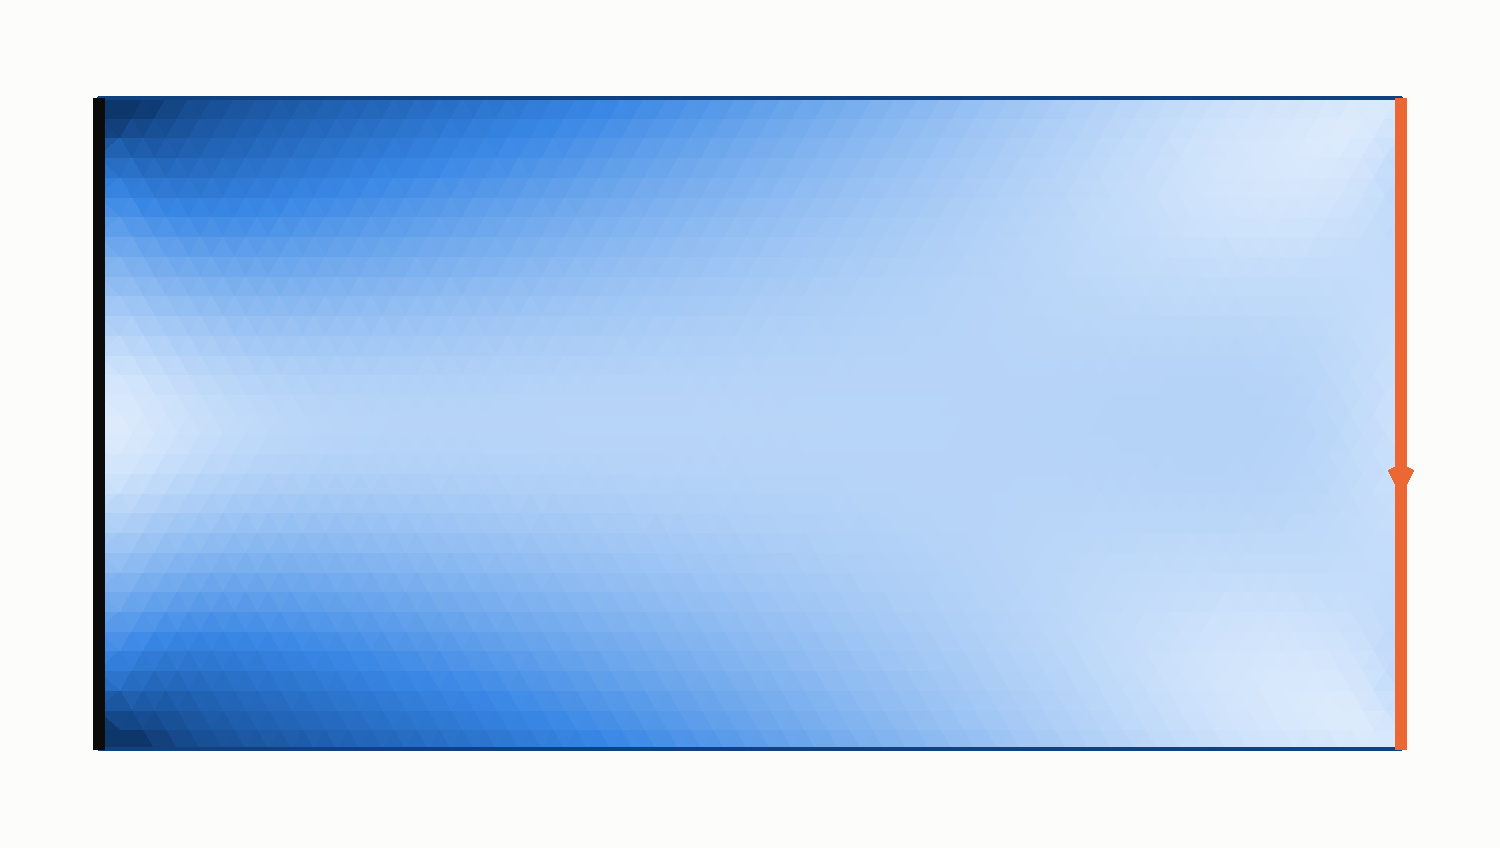
\includegraphics[width=1.00\textwidth]{figures/12_stress_bent.pdf}
\caption{The bent plate. Darker means higher stress. Held edge in black, loaded edge and force in orange. The top and bottom near the grip work hardest; the middle line and the free end hardly at all.}
\end{figure}
 

\begin{figure}[H]
\centering
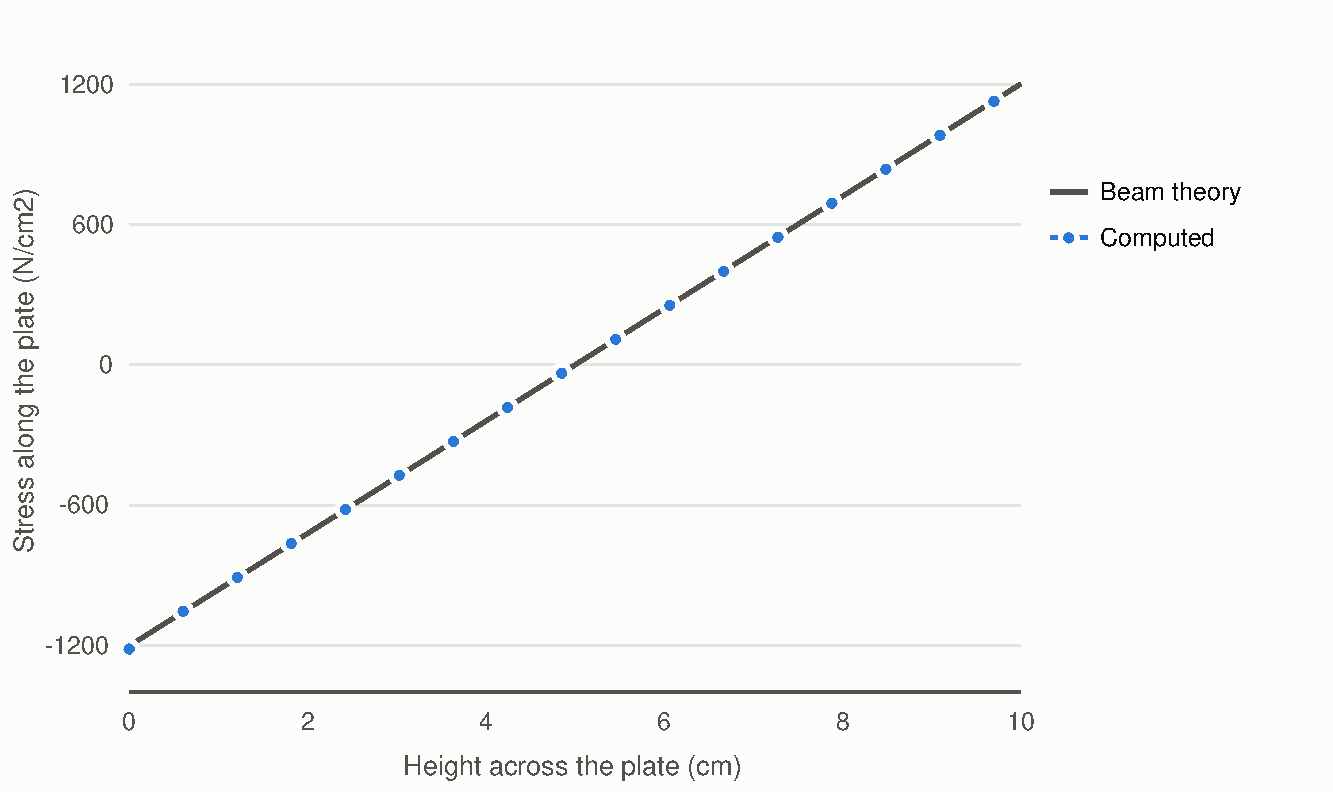
\includegraphics[width=0.80\textwidth]{figures/c_bending.pdf}
\caption{Stress along the plate across its height, half-way along. Points: computed. Line: beam theory, equation (23).}
\end{figure}
 

\subsection{A plate with a hole}
 

This is the classic test of a stress concentration. For a wide plate pulled with a far stress $\sigma _{\infty }$ and a round hole of radius $a$, on the line through the hole's centre across the pull, the stress in the pull direction at distance $r$ from the centre is (Kirsch) 
\begin{equation}
\frac{\sigma}{\sigma_\infty} = 1 + \frac{a^2}{2r^2} + \frac{3a^4}{2r^4}
\end{equation}
 

That is 3 on the rim, 1.65 at 0.4 $a$ from the rim and 1.22 at one radius from the rim. For a plate only ten radii wide the rim value rises to about 3.14. 

\begin{figure}[H]
\centering
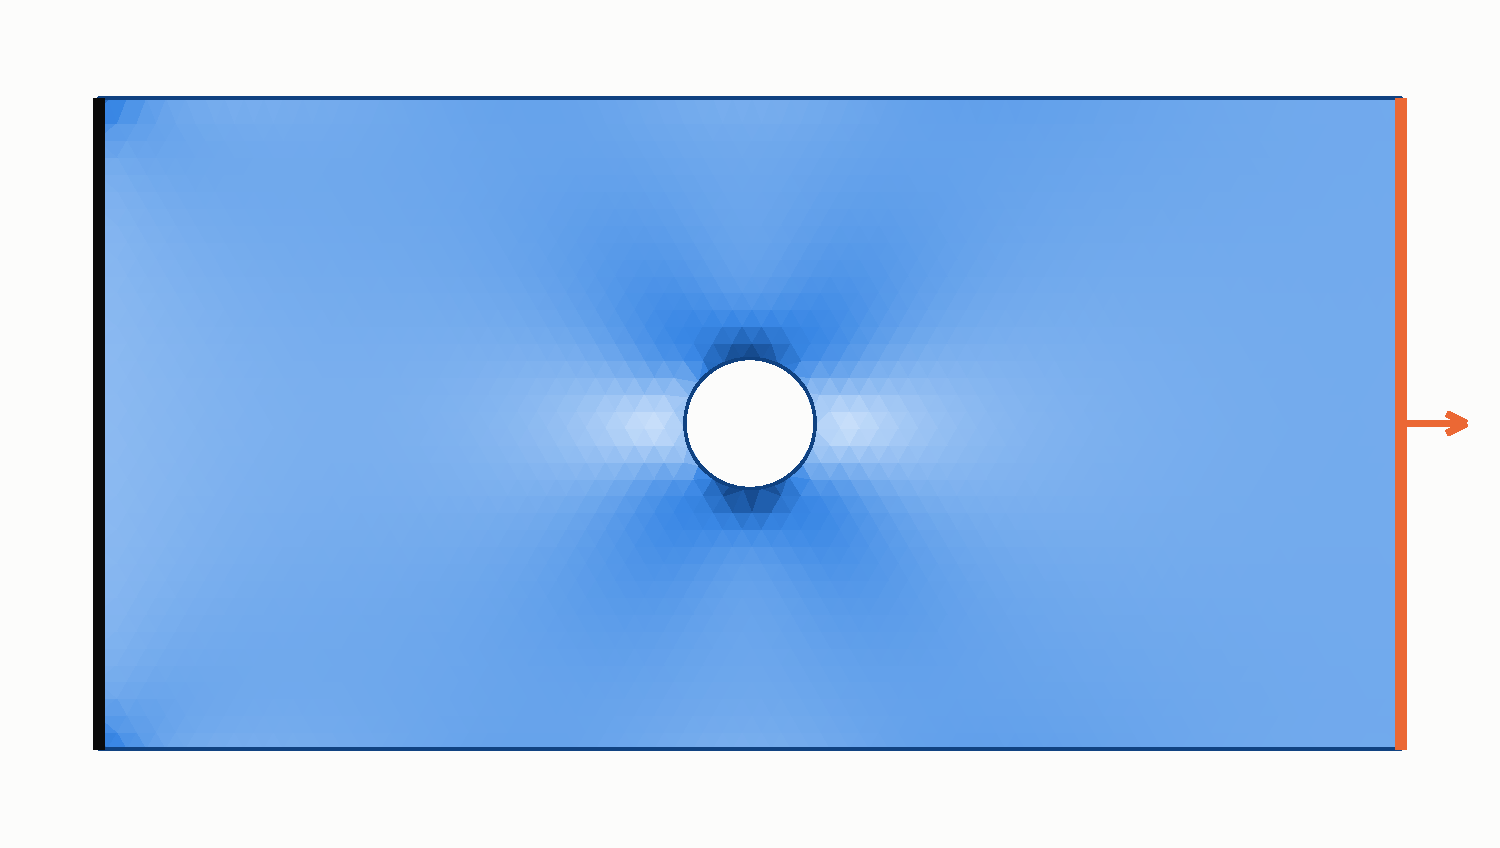
\includegraphics[width=1.00\textwidth]{figures/11_stress_hole.pdf}
\caption{A pulled plate with a hole. The stress concentrates beside the hole, across the pull, and falls away in front of and behind it.}
\end{figure}
 

\begin{figure}[H]
\centering
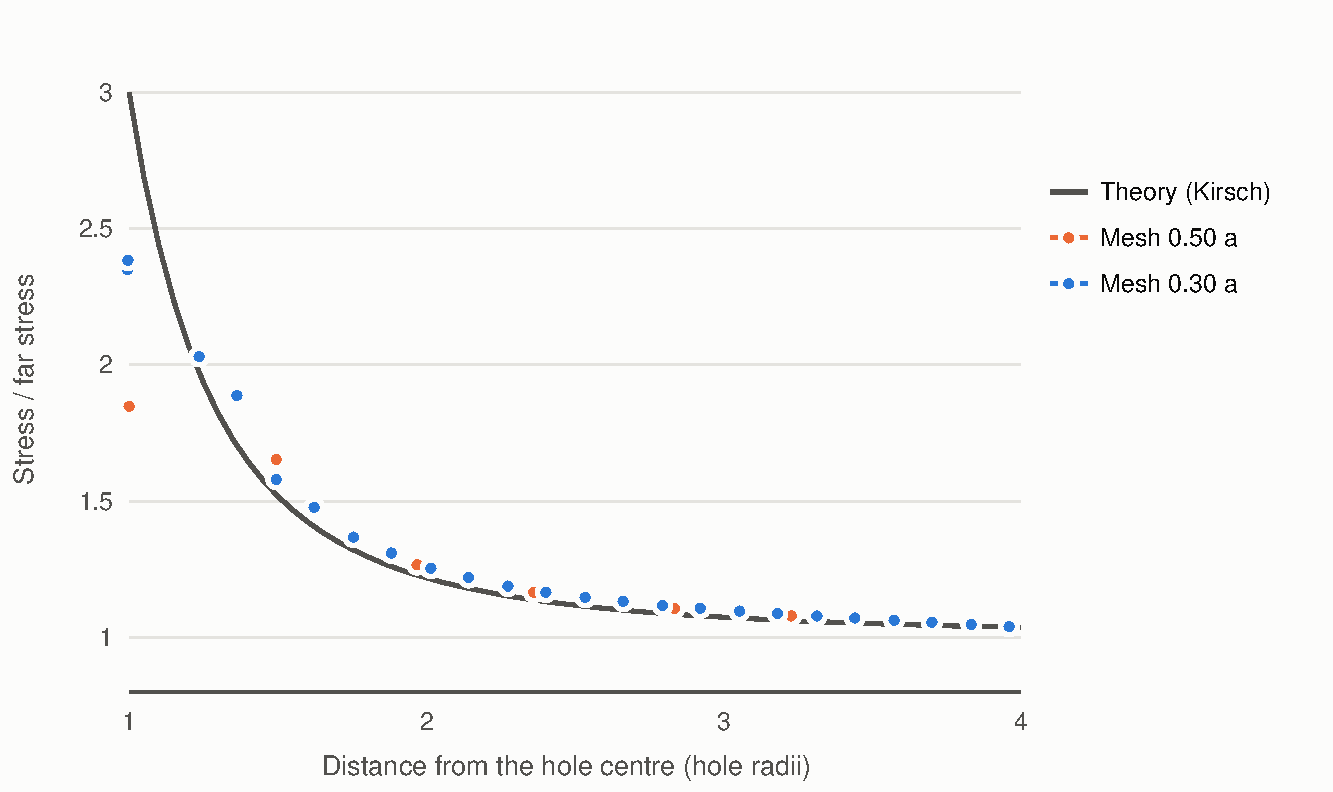
\includegraphics[width=0.80\textwidth]{figures/c_kirsch.pdf}
\caption{Stress against distance from the hole's centre, for two mesh sizes, against equation (24). From about 1.3 radii outward the computed points follow the theory. On the rim itself they fall short.}
\end{figure}
 

Figure 15 shows both the strength and the weakness of the method. Away from the rim the result is within about 5\% of theory on either mesh: 1.65 and 1.58 against 1.65 at 0.4 $a$ from the rim, 1.29 and 1.25 against 1.22 at one radius. Right on the rim the peak is underestimated, and it improves only slowly as the mesh gets finer. 

\begin{figure}[H]
\centering
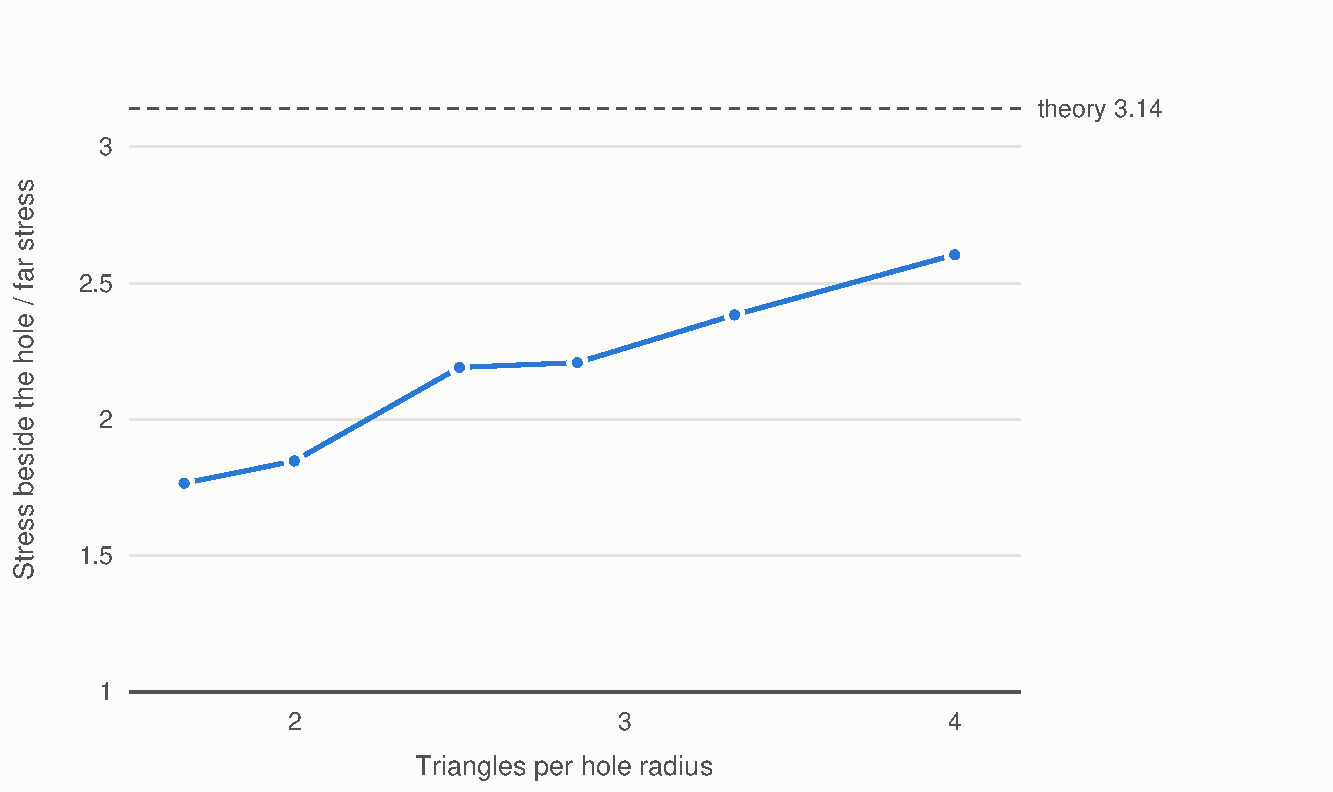
\includegraphics[width=0.80\textwidth]{figures/c_peak.pdf}
\caption{The computed stress beside the hole against the number of triangles per hole radius. At four triangles per radius it reaches 2.60 of the 3.14 that theory gives.}
\end{figure}
 

\begin{center}
\begin{tabular}{rrrr}
\toprule
Triangles per radius & Mesh points & Peak / far stress & Short of 3.14 by \\
\midrule
1.7 & 677 & 1.77 & 44\% \\
2.0 & 966 & 1.85 & 41\% \\
2.5 & 1,503 & 2.19 & 30\% \\
2.9 & 1,951 & 2.21 & 30\% \\
3.3 & 2,606 & 2.38 & 24\% \\
4.0 & 3,742 & 2.60 & 17\% \\
\bottomrule
\end{tabular}
\end{center}
 

The cause is the triangle itself. Its stress is constant across its area, so a sharp peak is spread over the neighbouring triangles. This is a well-known property of the simplest element type, and the plane fit at border points recovers only part of it. 

For steering a pocket pattern the weakness matters little: pockets start a border margin away from every edge, which is where the field is well resolved. As a statement about whether a part will hold, the peak value is not reliable, and the add-in says so. 

\subsection{A force at a point}
 

\begin{figure}[H]
\centering
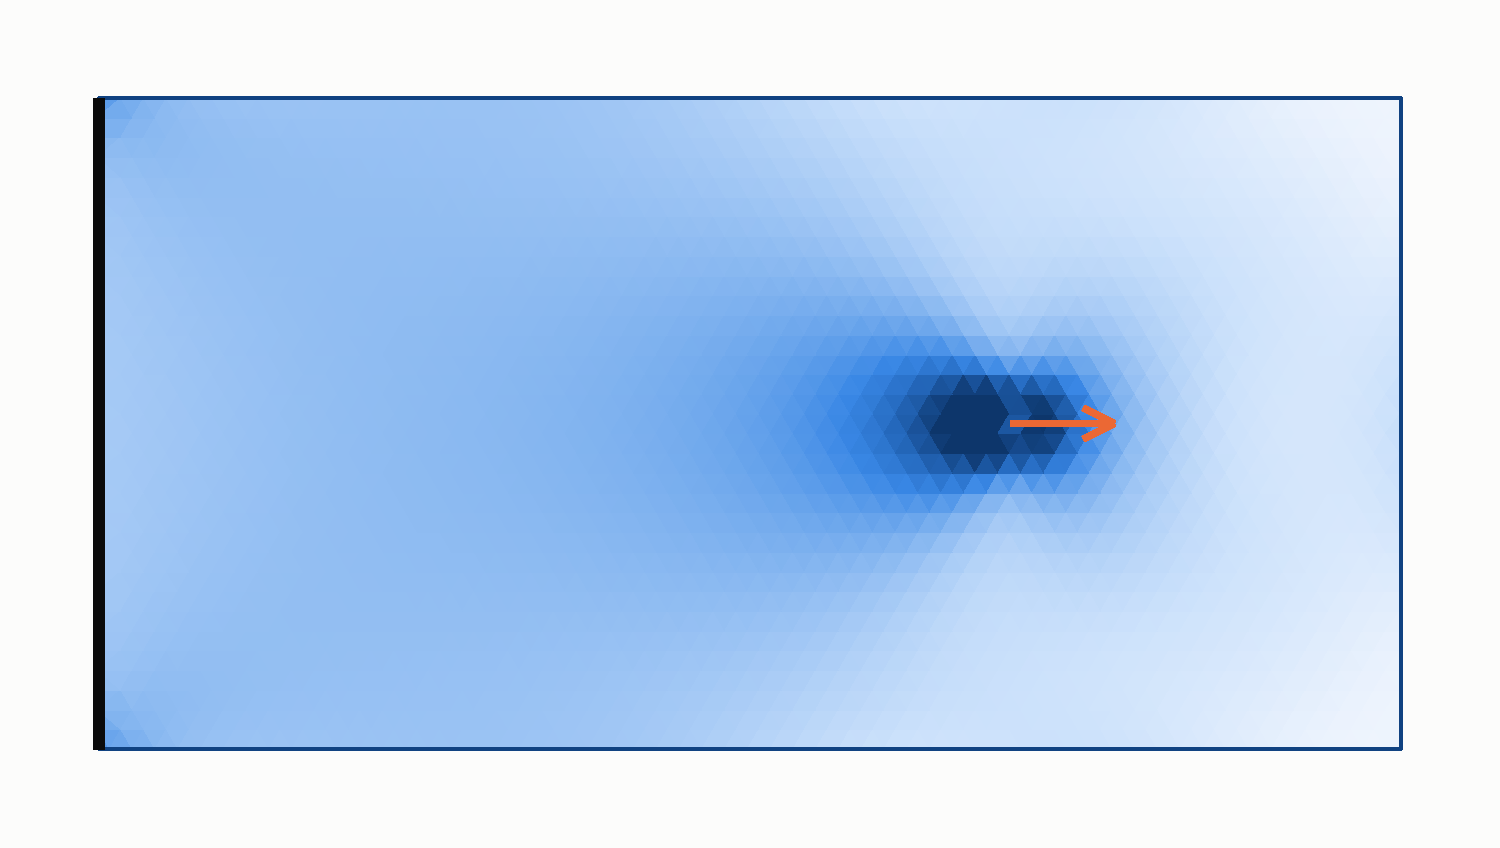
\includegraphics[width=1.00\textwidth]{figures/13_stress_point.pdf}
\caption{A plate held at its left edge and pulled to the right by 800 N at one point. The material behind the point is pulled, the material in front of it pushed.}
\end{figure}
 

Far from the point the pull has spread over the whole width: the computed stress near the grip is 163 N/cm$^2$ against 160 for an evenly pulled plate. Next to the point it rises to 719 N/cm$^2$. That figure depends on the spreading radius of equation (19) and should be read as "high here" rather than as a value. 

\section{Stress-driven patterns}
 

The stress field sets two things: how thick the walls of each cell are, and how large the cells are. 

\subsection{Wall thickness: keep material in proportion to load}
 

Suppose the solid plate carries the stress $\sigma $ at some spot, and after pocketing only the share $\kappa $ of the material is left there. If the remaining ribs carried the load as well as solid material, their stress would be about $\sigma $/$\kappa $. Requiring this to stay within the allowed stress gives the share that has to be kept: 
\begin{equation}
\kappa = \min\!\left(1,\; \frac{\sigma}{\sigma_{\mathrm{a}}}\right)
\end{equation}
 

A cell of size $s$ (the square root of its area) with walls $w$ loses a strip $w$/2 on every side, so its pocket covers about (1 $-$ $w$/$s$)$^2$ of it and the kept share is 1 $-$ (1 $-$ $w$/$s$)$^2$. Setting that equal to $\kappa $: 
\begin{equation}
w = s\left(1 - \sqrt{1 - \kappa}\right)
\end{equation}
 

For each cell, $\sigma $ is the highest stress found at the centroid and the corners of the cell (trimmed to the usable area), so a cell that touches a loaded zone is sized for it. The wall is never thinner than the thinnest wall chosen by the user. At $\kappa $ = 1 the cell stays solid; the code then uses a wall of 2$s$, which is larger than the widest circle that fits in any convex cell of that area and therefore leaves no pocket whatever the cell's shape. 

Each cell gives up half of its own wall on all sides, so the rib between two cells is the average of their two values and the thickness changes gradually across the plate. 

\begin{figure}[H]
\centering
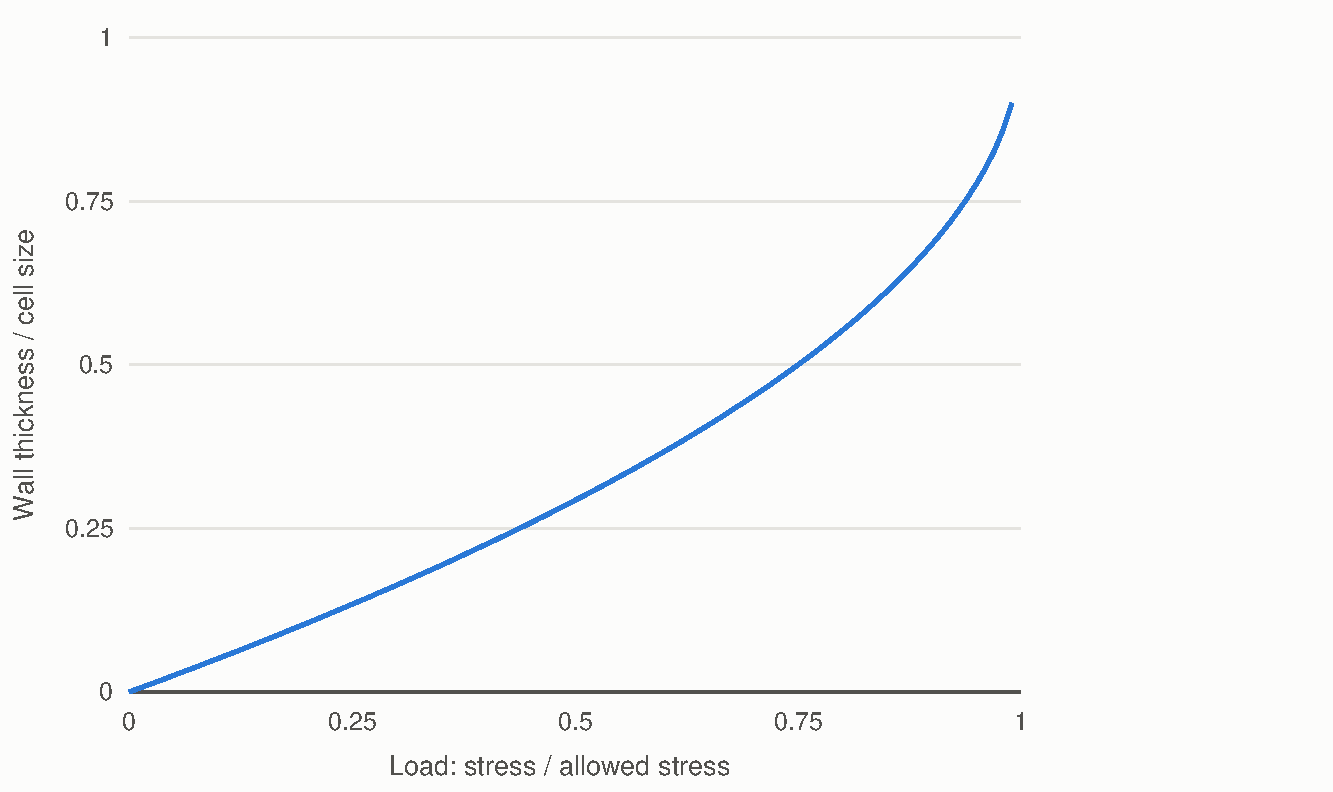
\includegraphics[width=0.80\textwidth]{figures/c_wall_rule.pdf}
\caption{Equation (26): wall thickness as a share of cell size, against load. Walls grow slowly at first and steeply near the allowed stress, where almost all material must stay.}
\end{figure}
 

\subsection{Cell size: small where busy, large where idle}
 

Cell size goes by how loaded a spot is compared with the rest of the same part, so the sizes always span the chosen range whatever the material. Let $\sigma _{5}$ and $\sigma _{95}$ be the values below which 5\% and 95\% of the mesh points lie; using these instead of the lowest and highest keeps one sharp peak from flattening everything else. With $R$ the chosen ratio between the widest and the narrowest cells: 
\begin{equation}
\beta = \operatorname{clamp}\!\left(\frac{\sigma - \sigma_5}{\sigma_{95} - \sigma_5},\; 0,\; 1\right)
\end{equation}
 
\begin{equation}
\omega = 1 - \left(1 - \frac1R\right)\beta, \qquad \rho = \frac{1}{\omega^2}
\end{equation}
 

The width changes evenly with the stress, from 1 where idle to 1/$R$ where busiest, and the number of cells per area is the inverse square of the width. If the part is loaded almost the same everywhere ($\sigma _{95}$ $-$ $\sigma _{5}$ below a tenth of $\sigma _{95}$), even cells are used. 

The seeds are thinned by $\rho $ as described in section 6. They are then evened out as in section 8, but each seed moves to the \emph{weighted} centre of its cell: 
\begin{equation}
\mathbf{x}_{\mathrm{new}} = \frac{\int \mathbf{x}\,\phi(\mathbf{x})\,\mathrm{d}A}{\int \phi(\mathbf{x})\,\mathrm{d}A}, \qquad \phi = \rho^2
\end{equation}
 

The weight is the density squared for a reason. Evening out pulls the spacing back toward uniform. For this kind of relaxation in two dimensions it is known that the points settle with a density proportional to the square root of the weight. Weighting by $\rho ^2$ therefore keeps them spread as $\rho $ itself asks. The integrals are approximated by cutting the trimmed cell into triangles from its centroid and taking the weight at the middle of each triangle. 

\subsection{Results}
 

\begin{figure}[H]
\centering
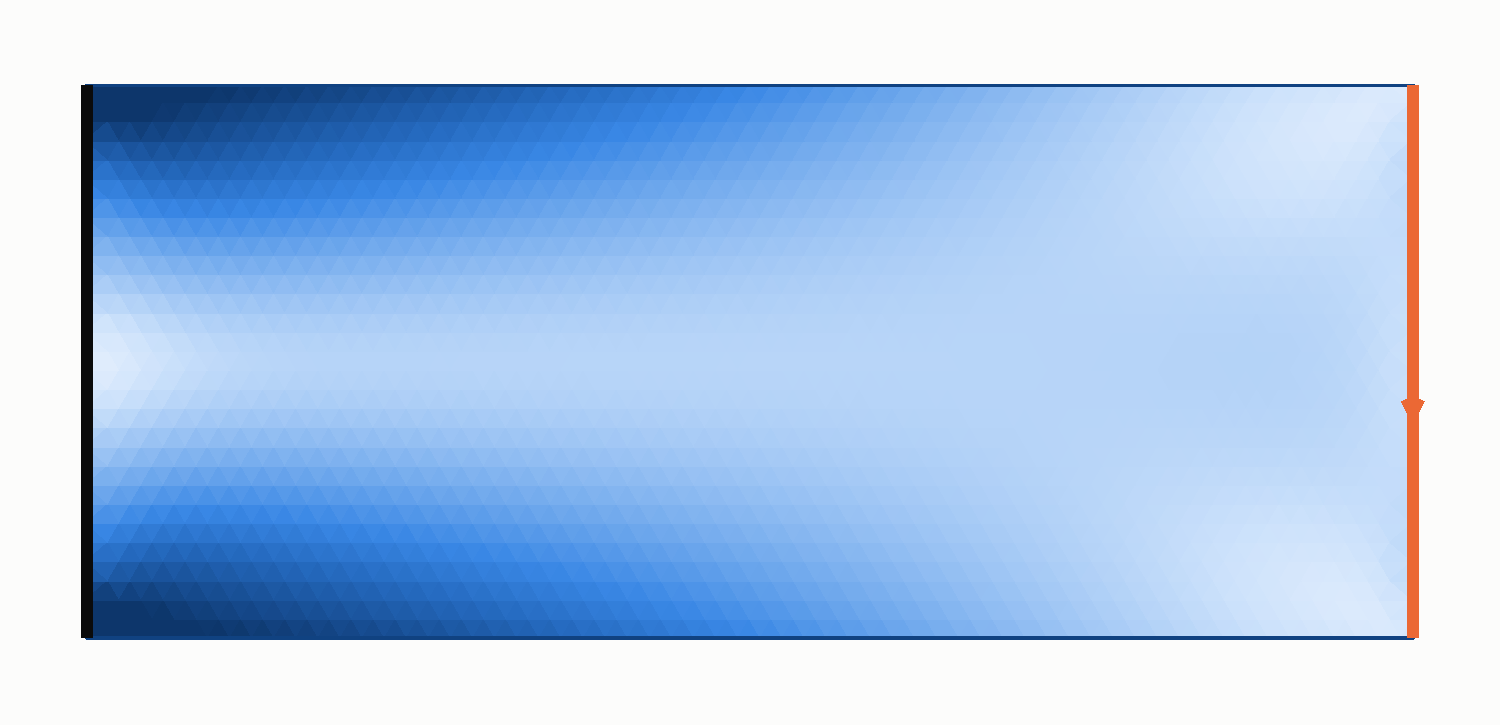
\includegraphics[width=1.00\textwidth]{figures/15_stress_bracket.pdf}
\caption{A bracket 240 $\times $ 100 $\times $ 5 mm, held at the left, pushed down at the right with 1000 N.}
\end{figure}
 

\begin{figure}[H]
\centering
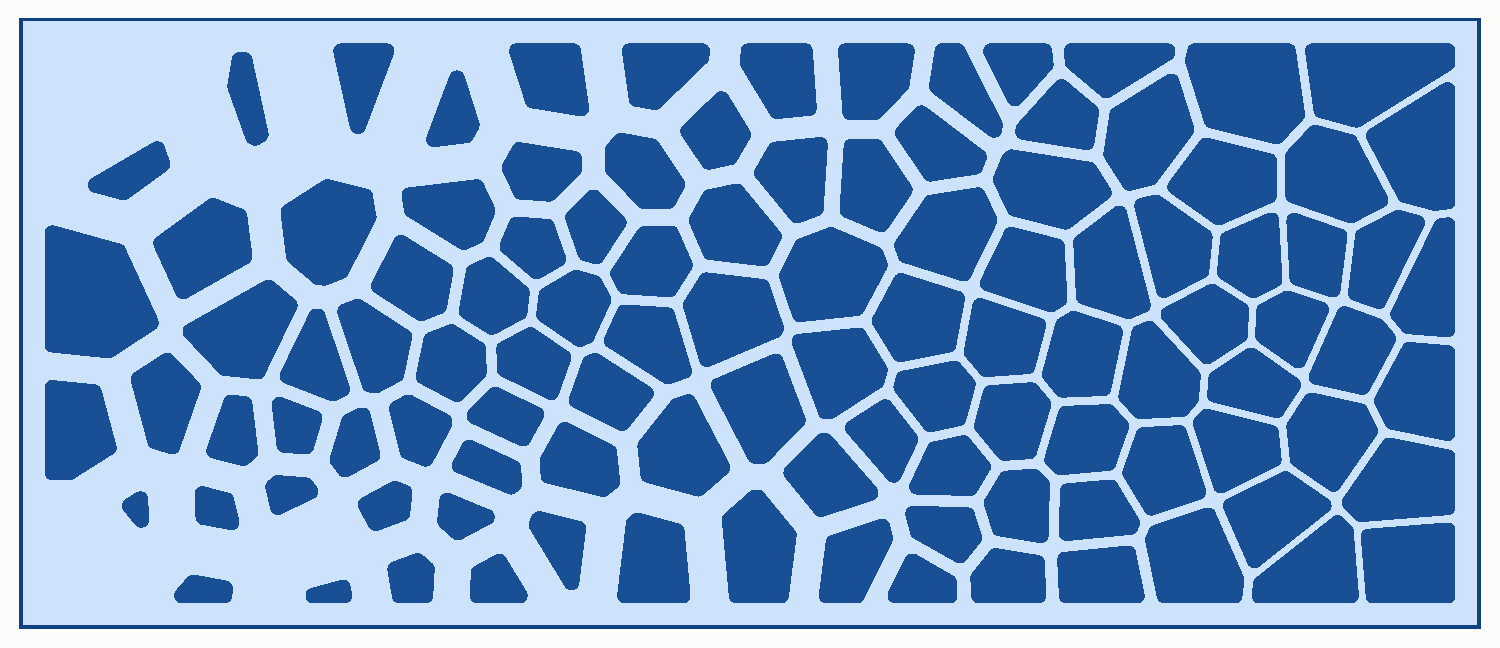
\includegraphics[width=1.00\textwidth]{figures/16_stress_even.pdf}
\caption{The pattern for Figure 19 with an allowed stress of 25 MPa and all cells the same size. Only the walls follow the stress: 1.2 mm at the idle end, growing toward the grip, with solid zones at the top and bottom corners where the stress exceeds the allowed value.}
\end{figure}
 

\begin{figure}[H]
\centering
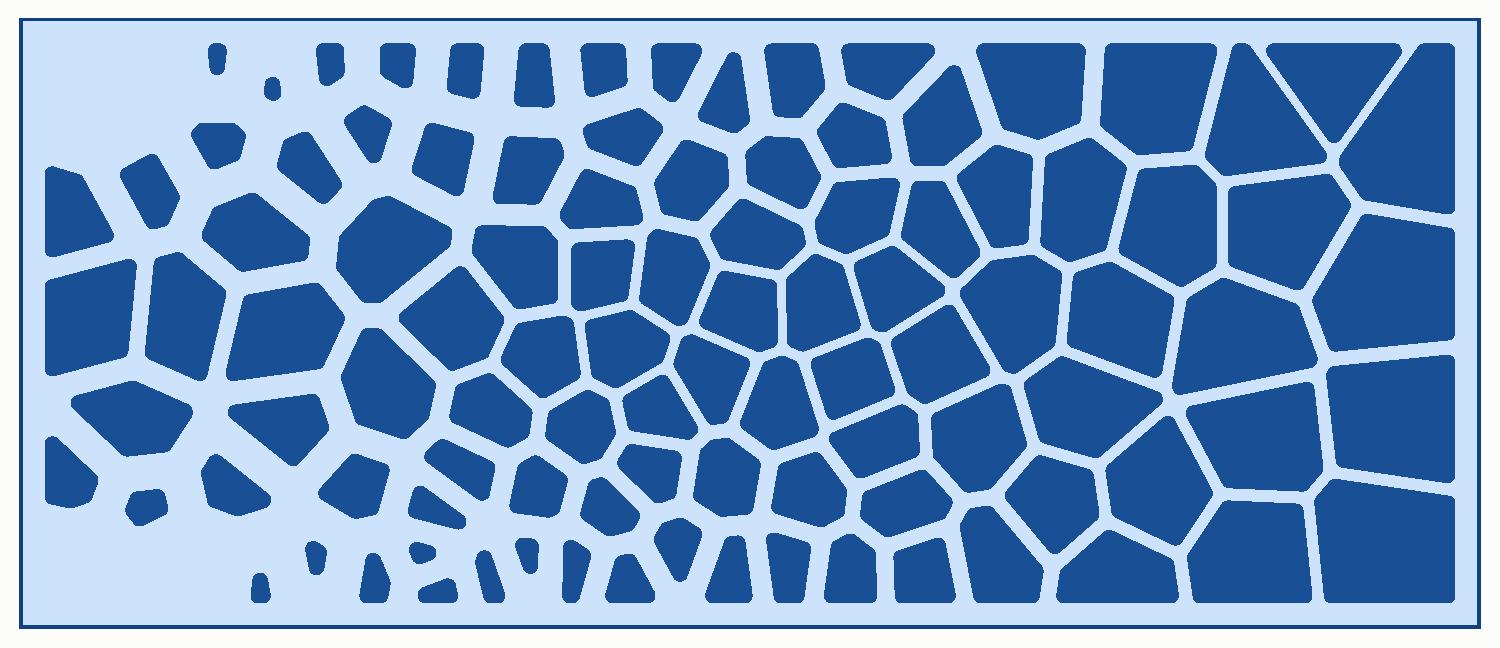
\includegraphics[width=1.00\textwidth]{figures/17_stress_varied.pdf}
\caption{The same with a size ratio of 2.5. Cells are 7 mm wide near the grip and 22 mm wide at the idle end. The number of cells is the same as in Figure 20; they have moved to where the load is.}
\end{figure}
 

\begin{figure}[H]
\centering
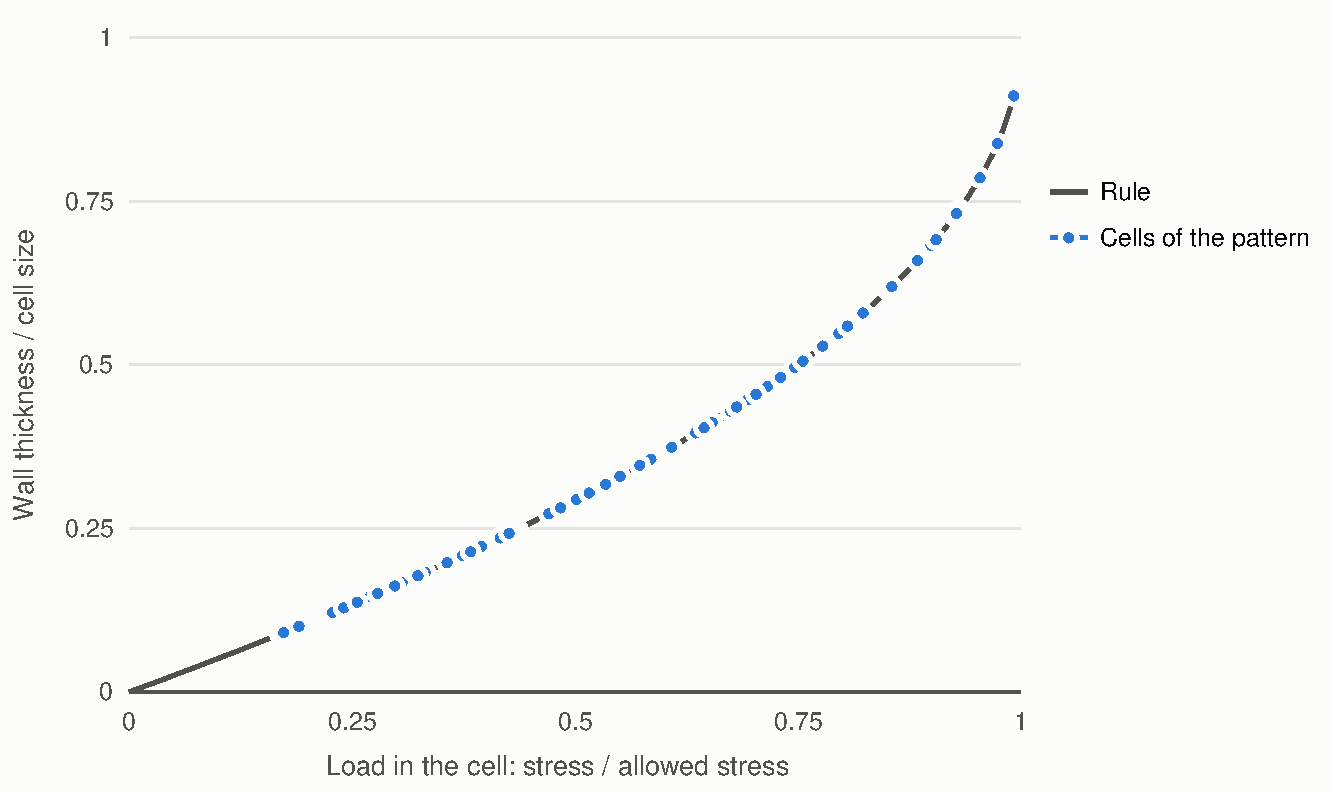
\includegraphics[width=0.80\textwidth]{figures/c_wall_cells.pdf}
\caption{Every cell of Figure 21: its wall thickness over its size against its load. Cells on the curve follow equation (26). A cell lies above the curve where the thinnest allowed wall is more than the rule asks for.}
\end{figure}
 

\begin{figure}[H]
\centering
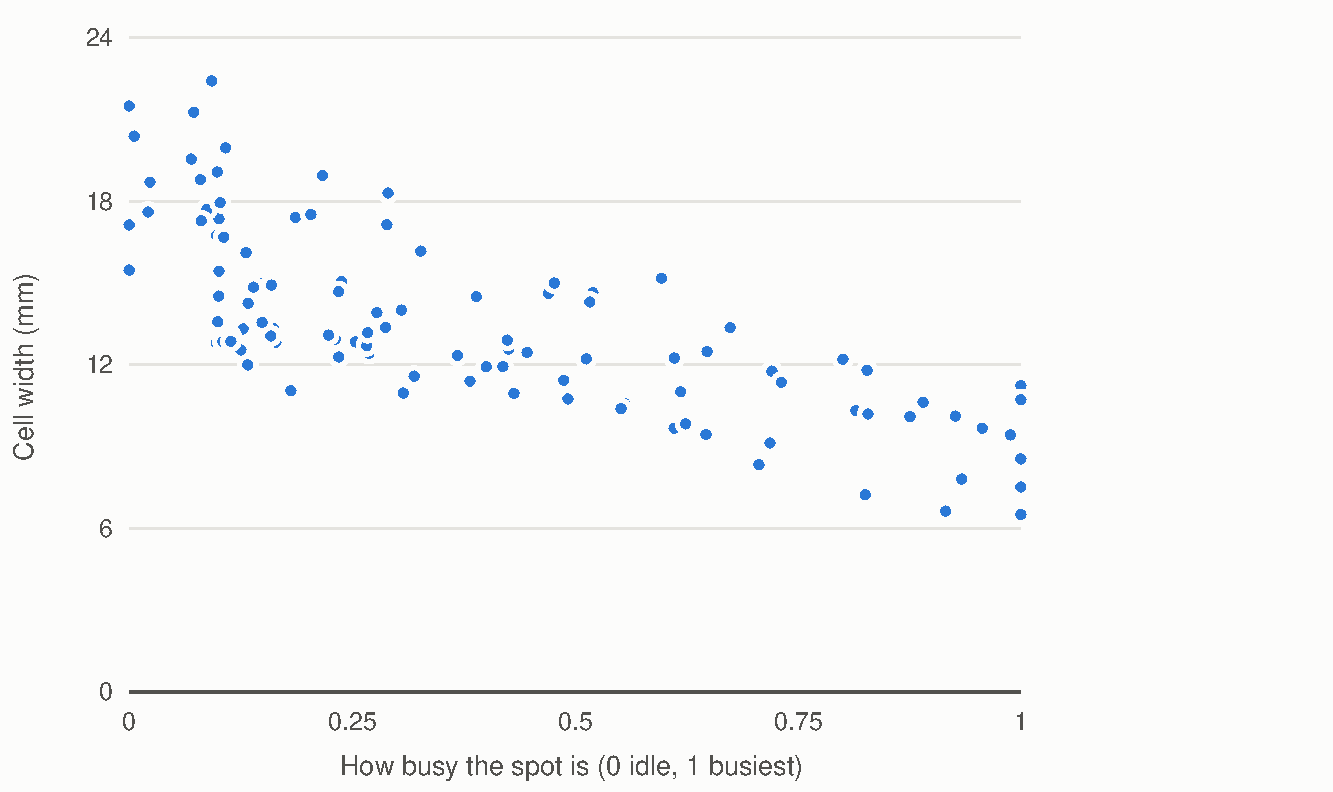
\includegraphics[width=0.80\textwidth]{figures/c_size_cells.pdf}
\caption{Cell width against how busy the spot is, for the cells of Figure 21. The widths fall from about 20 mm to about 8 mm, with the scatter that comes from random seeding and only three smoothing passes.}
\end{figure}
 

\begin{figure}[H]
\centering
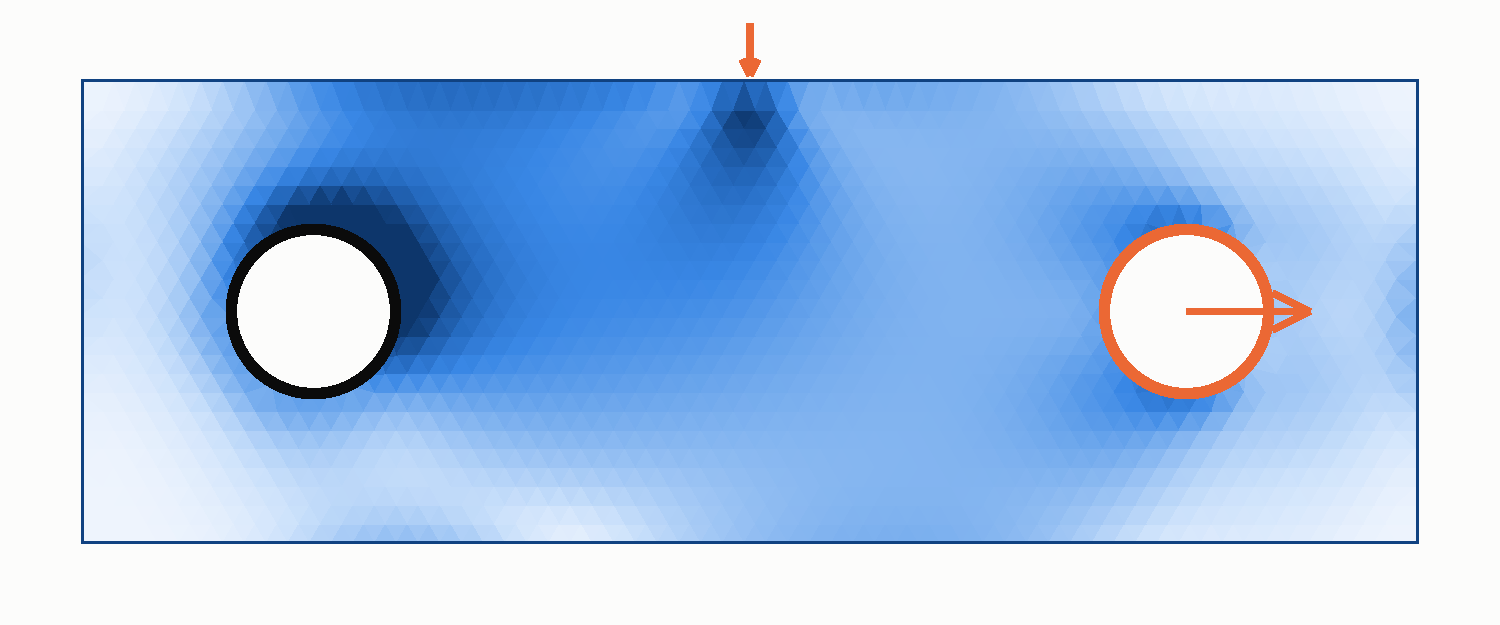
\includegraphics[width=1.00\textwidth]{figures/18_stress_link.pdf}
\caption{A link held at its left hole (black rim), pulled at its right hole with 4000 N and pushed down at the middle of its top edge with 1500 N.}
\end{figure}
 

\begin{figure}[H]
\centering
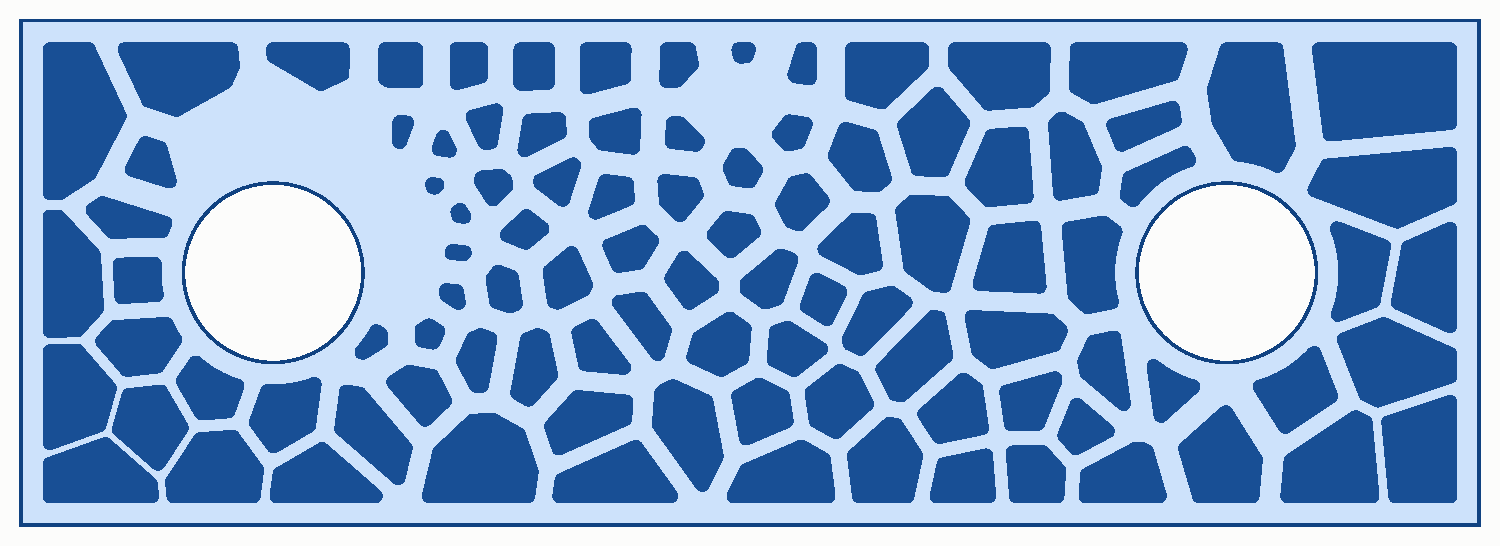
\includegraphics[width=1.00\textwidth]{figures/19_pattern_link.pdf}
\caption{The pattern for Figure 24: 99 pockets covering 48\% of the face. Material stays where the forces enter and along the path between the holes; the corners far from the load path get the largest pockets.}
\end{figure}
 

\section{Speed}
 

All times are for plain Python on the development machine and are meant to show how the cost grows, not as benchmarks. They vary by about a tenth from run to run. 

\subsection{Pattern}
 

\begin{figure}[H]
\centering
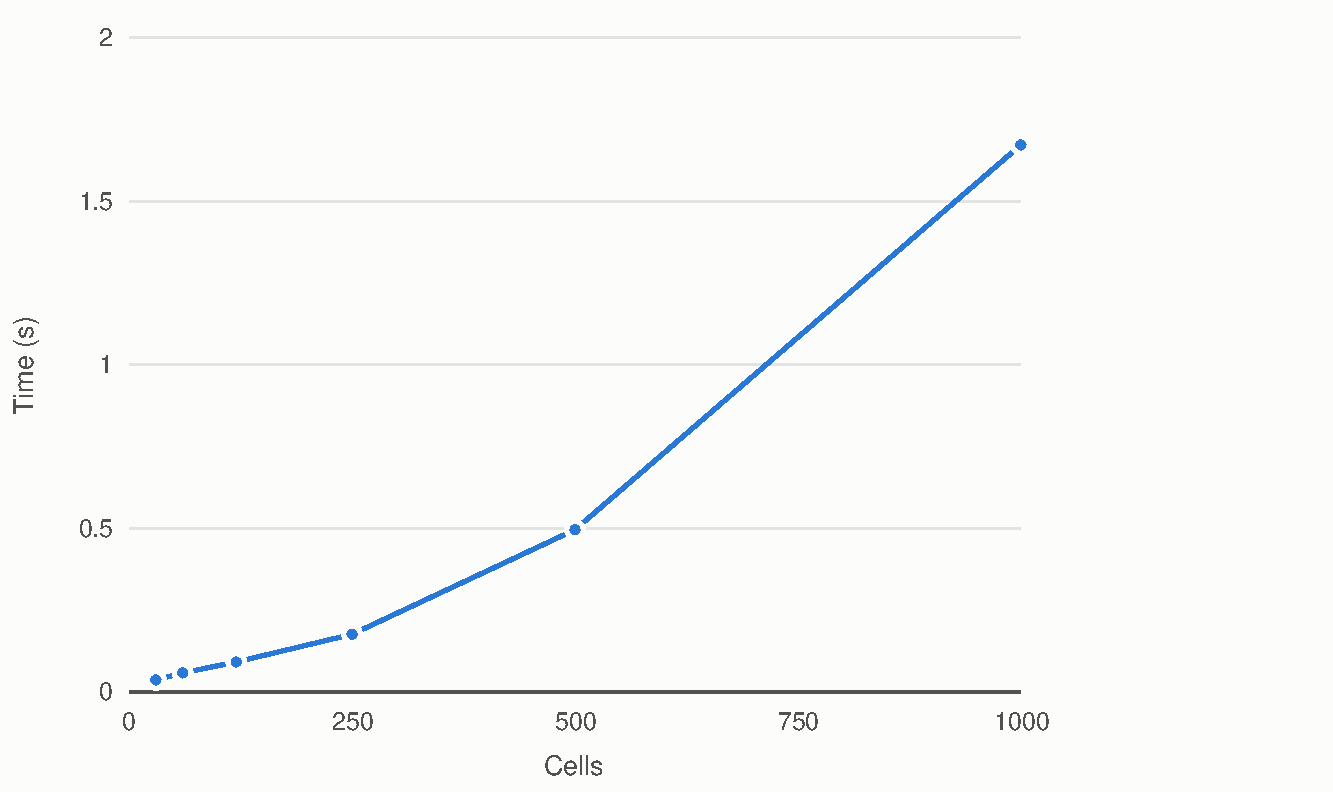
\includegraphics[width=0.80\textwidth]{figures/c_pattern_time.pdf}
\caption{Time for a complete pattern on the example face against the number of cells: 0.06 s for 60 cells, 0.5 s for 500, 1.7 s for 1,000.}
\end{figure}
 

The curve bends upward because each Voronoi cell sorts all other seeds by distance, which costs more per cell as the count grows. Up to a few hundred cells this is negligible. Simple mode costs more, 0.5 to 0.7 s, because it repeats the last three steps about sixteen times over a few cell counts. 

Three measures keep the trimming step, where most of the time goes, cheap: cells away from every edge skip it after one inside test; the edges of a region are found through the grid of section 5 rather than by looking at all of them; and the inside test for pieces of one loop is done once per unbroken run. Together they roughly halved the time of simple mode. 

\subsection{Stress}
 

\begin{figure}[H]
\centering
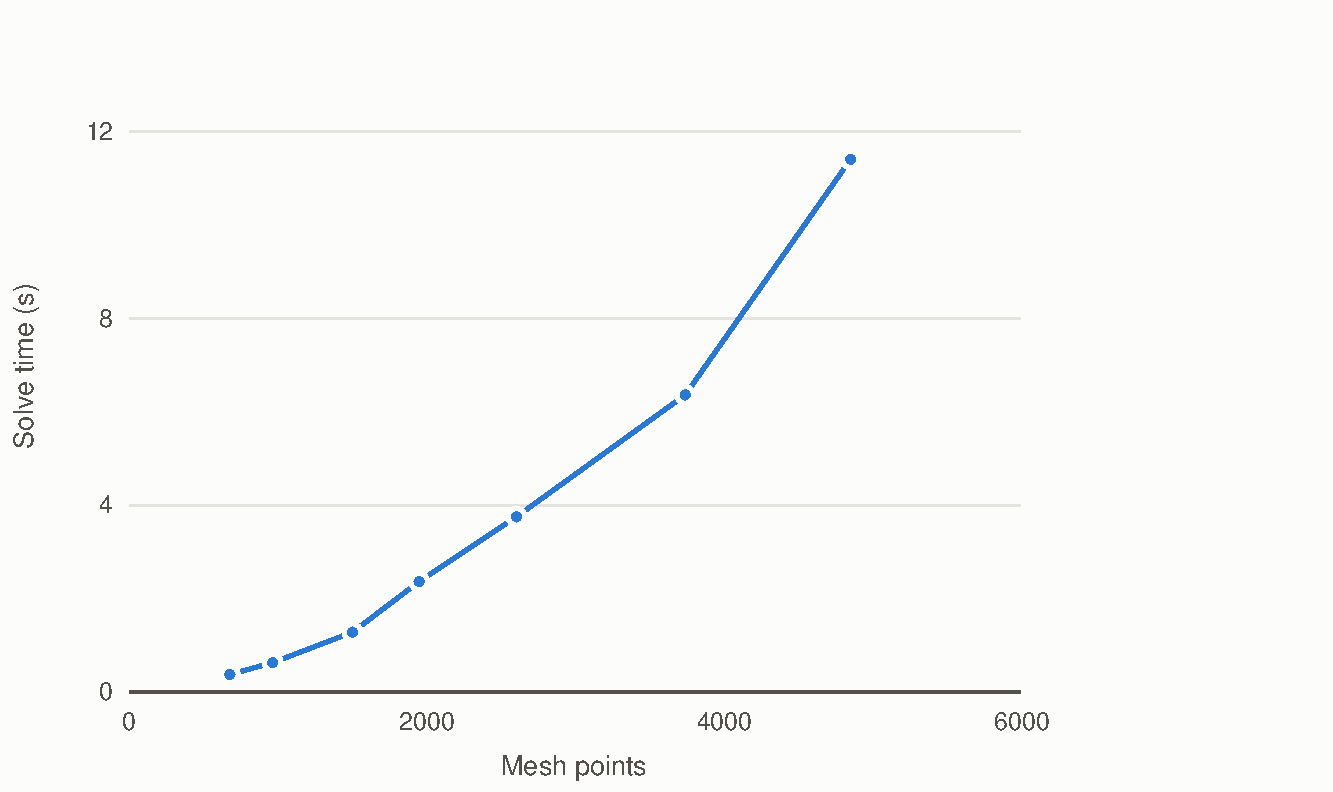
\includegraphics[width=0.80\textwidth]{figures/c_solve_time.pdf}
\caption{Time for one stress calculation against the number of mesh points.}
\end{figure}
 

\begin{figure}[H]
\centering
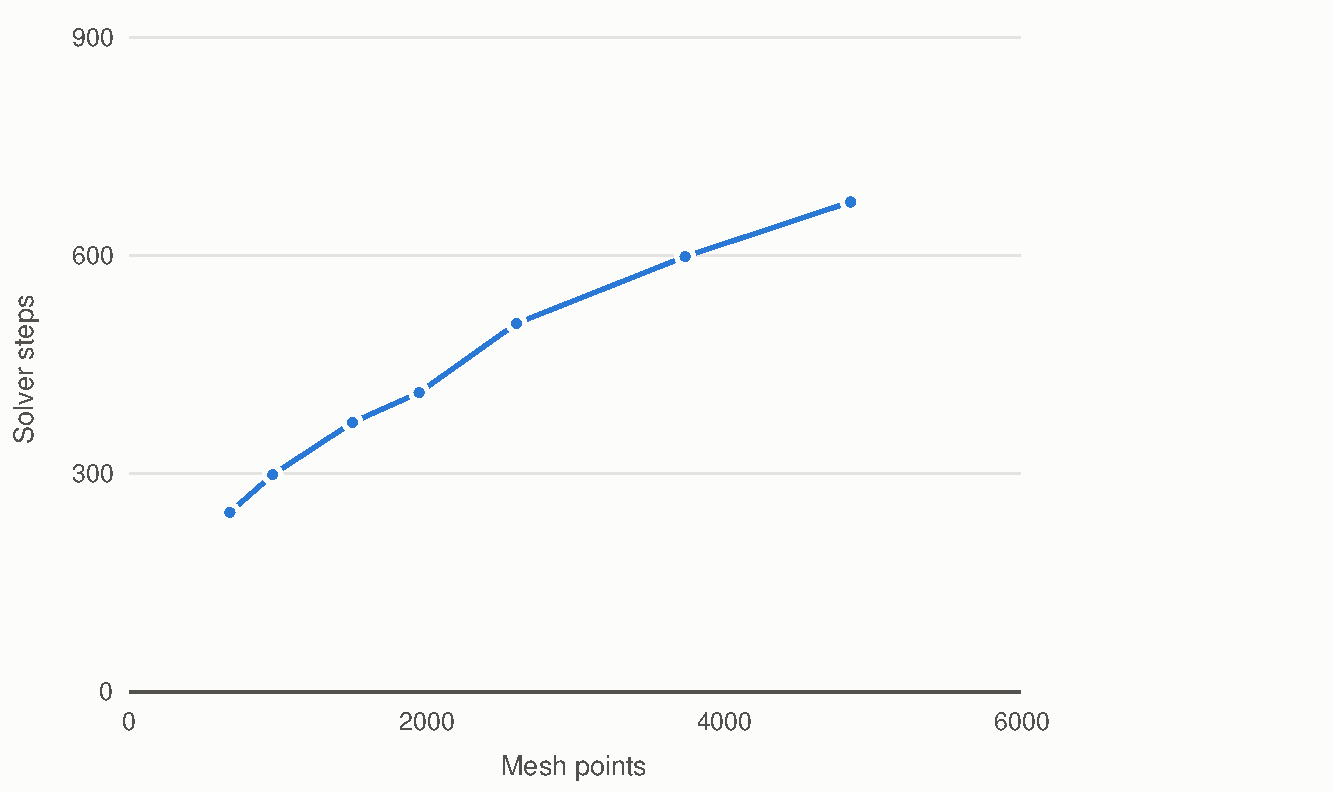
\includegraphics[width=0.80\textwidth]{figures/c_solve_steps.pdf}
\caption{Solver steps against the number of mesh points.}
\end{figure}
 

\begin{center}
\begin{tabular}{rrr}
\toprule
Mesh points & Solver steps & Time (s) \\
\midrule
677 & 247 & 0.4 \\
966 & 299 & 0.6 \\
1,503 & 371 & 1.3 \\
1,951 & 412 & 2.4 \\
2,606 & 507 & 3.8 \\
3,742 & 599 & 6.4 \\
4,854 & 674 & 11.4 \\
\bottomrule
\end{tabular}
\end{center}
 

The work per step is proportional to the number of points, and the number of steps grows roughly with its square root, so the time grows faster than the mesh. The default mesh of about 2,500 points is the largest that still answers in two to three seconds. The stress is computed once and reused until a support, a force or the thickness changes; changing the pattern settings or the pocket depth does not repeat it. 

This is the one part of the method where plain Python sets the limit on quality: the mesh that would resolve the peak beside a hole (Figure 16) is out of reach at interactive speed. 

\section{How it is tested}
 

The method is covered by 65 automated tests of the mathematics, which run without the host program. Rather than comparing against stored results, most of them check a property that must hold. 

\begin{center}
\begin{tabular}{>{\raggedright\arraybackslash}p{0.27\textwidth}>{\raggedright\arraybackslash}p{0.65\textwidth}}
\toprule
What & How it is checked \\
\midrule
Shrinking a region & For thousands of random points: the point is inside the shrunk region exactly when it is on the face and at least the distance from every edge. Run on an L-shape, faces with holes, a curved outline, a hole close to the edge, a neck that pinches off and an arm that vanishes. \\
Trimming a cell & For random points: inside the result exactly when inside both the cell and the region. Run on an inward corner, a result in two pieces, a hole inside the cell, a grown hole overlapping the outline, and 25 random boxes on the curved outline. \\
Voronoi cells & The cells tile the box (their areas add up to its area), each contains its seed, and no other seed is closer to any cell corner. \\
Patterns & Every pocket point is on the face and at least the margin from every edge; every pair of pockets is at least the wall apart; every arc has exactly the corner radius; with no wall and no margin the pockets fill the face exactly. \\
Simple mode & The share reached is within 0.5\% of the share asked for on four faces; walls land within 20\% of the margin when the cell count is free; an unreachable share is reported. \\
Stress & The exact and textbook cases of section 15, the balance between applied force and support reaction, and that stress scales with force and does not change with stiffness. \\
Stress-driven patterns & Walls of the busiest quarter of cells are at least three times those of the idlest quarter; cells are clearly smaller where loaded; with no load the pattern equals the ordinary one. \\
\bottomrule
\end{tabular}
\end{center}
 

\section{Limits}
 
\begin{itemize}
 
\item \textbf{The stress is that of the solid plate.} Cutting the pockets changes the stress field, and this is not fed back. The safety factor shown is the solid plate's. Checking the pocketed plate would need a mesh fine enough for the thinnest walls, far beyond the sizes in section 17. 
\item \textbf{The wall rule is optimistic.} Equation (25) assumes the ribs carry load as well as solid material. Ribs at an angle to the load carry less, and a random cell structure deforms partly by bending of its walls. The target safety factor has to cover this. 
\item \textbf{Peaks read low} at hole rims and sharp inward corners (Figure 16), and the stress under a point force depends on its spreading radius. 
\item \textbf{In-plane only.} Forces out of the face's plane, bending of the plate, and the floor left under pockets that do not go through are not part of the model. 
\item \textbf{One mesh size.} Triangles are the same size everywhere; there is no refinement near holes and corners. 
\item \textbf{Curved pocket sides are polylines.} Where a pocket follows a curved edge, that side consists of short straight pieces within 0.02 mm of the true curve. 
\item \textbf{C-shaped holes.} If growing a hole closes it into a ring, the island of material inside is treated as part of the hole and gets no pockets. 
\end{itemize}
 

\begin{quote}
The stress-driven mode is a way to put material where the load is. It is not a strength check. A part that matters should be verified with a full simulation of the finished, pocketed shape.
\end{quote}

\section*{Further reading}

\begin{itemize}
  \item O.~C. Zienkiewicz, R.~L. Taylor, J.~Z. Zhu, \emph{The Finite Element Method: Its Basis and
        Fundamentals}, Butterworth-Heinemann. (The triangle element of section~14.)
  \item S.~P. Timoshenko, J.~N. Goodier, \emph{Theory of Elasticity}, McGraw-Hill. (Plate with a hole.)
  \item W.~D. Pilkey, D.~F. Pilkey, \emph{Peterson's Stress Concentration Factors}, Wiley.
        (A hole in a plate of finite width.)
  \item M.~R. Hestenes, E.~Stiefel, Methods of conjugate gradients for solving linear systems,
        \emph{J. Res. Natl. Bur. Stand.} 49 (1952).
  \item Q.~Du, V.~Faber, M.~Gunzburger, Centroidal Voronoi tessellations: applications and algorithms,
        \emph{SIAM Review} 41 (1999). (Evening out seed points, with and without weights.)
\end{itemize}

\end{document}
